% Esta es la Plantilla UNAL en LaTeX
\documentclass[10pt,spanish,fleqn,openany,twoside,letterpaper]{book}

%Muestra los márgenes del documento para evitar Warnings
%Para activar la siguiente línea quite el simbolo % 
%\usepackage[showframe]{geometry}

%Formato de fuentes bibliográficas
%Use el estilo bibliográfico que sea pertinente según el área de estudio APA, IEEE, etc

%Usando el paquete BibLaTeX
%Cita normal con \cite[página]{} y cita con paréntesis \parencite[página]{}

% Configuración de BibLaTeX
%\usepackage[backend=biber,style=authoryear,maxcitenames=2,maxbibnames=99,giveninits=true,uniquename=false]{biblatex}
%\addbibresource{biblio.bib}

% Cambiar el idioma de las referencias bibliográficas a español
%\DefineBibliographyStrings{spanish}{%
%  andothers = {et\addabbrvspace al\adddot},
%  andmore = {et\addabbrvspace al\adddot},
%}

% Personalizar el formato de las citas y la bibliografía
%\DeclareNameAlias{sortname}{family-given}
%\DeclareDelimFormat{multinamedelim}{\addcomma\space}
%\DeclareDelimFormat{finalnamedelim}{\addcomma\space\&\space}
%\DeclareFieldFormat{titlecase}{\MakeSentenceCase*{#1}}
%\DeclareFieldFormat[article,inbook,incollection,inproceedings,patent,thesis,unpublished]{title}{\titlecase{#1}}
%\DeclareFieldFormat{journaltitlecase}{\titlecase{#1}}
%\DeclareFieldFormat{pages}{#1}
%\DeclareFieldFormat{volume}{\mkbibbold{#1}}
%\renewbibmacro{in:}{}
%\AtEveryBibitem{\clearfield{month}}

%Usando el paquete Natbib
%Cita normal \cite[página]{} y cita con paréntesis \citep[página]{}
\usepackage{natbib}
\bibpunct{[}{]}{;}{\&}{.}{}
\bibliographystyle{dtvstyle}

%Idioma del documento
%Use main para el idioma principal del documento
\usepackage[main=spanish,english,german,french,portuguese]{babel}

% Carácteres especiales
\usepackage{fontenc}

\usepackage[export]{adjustbox}

% Evita ligadura li & fl
\usepackage{microtype}
\DisableLigatures{encoding = *, family = *}

% Otros paquetes de tablas y colores avanzados
\usepackage{amsmath,graphicx,rotating,float,multirow}
%\usetikzlibrary{positioning}
\usepackage{longtable}
\setlength{\LTcapwidth}{6in}
\usepackage[utf8]{inputenc}
\usepackage{epsfig,epic,eepic,threeparttable,amscd,here,lscape,tabularx,subcaption}
\usepackage{tabu,array}
\usepackage[rgb]{xcolor}

\usepackage{tikz}
\usetikzlibrary{shapes, arrows.meta, positioning}
% Permite ver y configurar los parámetros de la página
\usepackage{layout}
%Hyperref permite ver las secciones del texto
\usepackage[hidelinks]{hyperref}

%Permite incluir código de cualquier lenguaje dentro del texto del documento
\usepackage{minted}
\usepackage{float}
\usepackage{fancyvrb}
\usepackage{pgfplots}
\usepackage{pgfplotstable}
\usepackage{booktabs}
\usepackage{svg}
\pgfplotsset{compat=1.18}
\usepackage{xcolor}
\newenvironment{myverbatim}{\Verbatim}{\endVerbatim}

%Genera los comandos de la página de autoría
\newcommand{\studentname}{}
\newcommand{\submissiondate}{}
\newcommand{\academictitle}{}
\newcommand{\resgroupone}{}
\newcommand{\resgrouptwo}{}
\newcommand{\researchtopic}{}
\newcommand{\thesisname}{}
\newcommand{\thesisnameeng}{}
\newcommand{\thesisnamelang}{} %Usar solo si se requiere
\newcommand{\director}{}
\newcommand{\directortitle}{}
\newcommand{\codirector}{} %Usar solo si se requiere
\newcommand{\codirectortitle}{} %Usar solo si se requiere
\newcommand{\issuedate}{}
\newcommand{\palabrasclave}{}
\newcommand{\keywords}{}
\newcommand{\schlusselworter}{}
\newcommand{\palavraschave}{}
\newcommand{\sede}{}
\newcommand{\department}{}
\newcommand{\departmenttwo}{} %Usar solo si se requiere
\newcommand{\faculty}{}
\newcommand{\university}{Universidad Nacional de Colombia}

%Información de la tesis
%Diligenciar aquí los datos para su carga automática donde se requiera en el documento
%En el caso de tesis o trabajos finales, verificar que el título coincida con el aprobado por la Facultad
\renewcommand{\studentname}{Juan Pablo Vargas Acosta}
\renewcommand{\thesisname}{Estudio de desempeño para conjuntos de ejemplares de herbarios de modelos de vision por computador en esquema federado}
\renewcommand{\thesisnameeng}{Performance study on sets of samples from herbariums of computer vision models on a federated scheme}
%\renewcommand{\thesisnamelang}{Nombre del trabajo o tesis en un tercer idioma} %Usar solo si se requiere
\renewcommand{\issuedate}{2025}
\renewcommand{\submissiondate}{Julio}
\renewcommand{\director}{Prof. Dr. Director Francisco Gomez}
\renewcommand{\directortitle}{Titular}
\renewcommand{\codirector}{Prof. Dr. Co director Lauren Rz}
\renewcommand{\codirectortitle}{Titular}
\renewcommand{\academictitle}{Magíster (M, MSc) }
\renewcommand{\resgroupone}{COMBIOS}
%\renewcommand{\resgrouptwo}{Grupo B (Sigla Grupo Investigación 02) }
\renewcommand{\researchtopic}{Matematicas Aplicadas : Vision Por Computador}
\renewcommand{\sede}{Bogota} 
\renewcommand{\department}{Matematicas}
\renewcommand{\departmenttwo}{Biologia} %Usar solo si es necesario
\renewcommand{\faculty}{Ciencias}

%Palabras clave del documento - Tener presente los Theasurus https://www.thesaurus.com/
%Disponible en 3 idiomas aunque se puede extender a francés o otro idioma
\renewcommand{\palabrasclave}{Visión por Computadora, Aprendizaje Federado, YOLO, ResNet, CNN (Redes Neuronales Convolucionales), Herbario Digital, Identificación de Features en la Imagen, Segmentación de Imágenes, Clasificación de Sellos y Anotaciones, Transfer Learning, Fine-Tuning de Modelos, mAP (Mean Average Precision), Preprocesamiento de Imágenes, Feature Extraction, Adaptación de Modelos Preentrenados.} 
\renewcommand{\keywords}{Computer Vision, Federated Learning, YOLO, ResNet, CNN (Convolutional Neural Networks), Digital Herbarium, Feature Identification in Images, Image Segmentation, Stamp and Annotation Classification, Transfer Learning, Fine-Tuning of Models, mAP (Mean Average Precision), Image Preprocessing, Feature Extraction, Pretrained Model Adaptation.}
%\renewcommand{\schlusselworter}{}
%\renewcommand{\palavraschave}{}

% Estilo de los encabezados y pies de página
\usepackage{fancyhdr}
\fancyhf{}%
\pagestyle{fancyplain}
\textheight22.5cm \topmargin0cm \textwidth16.5cm \headheight22pt
\oddsidemargin0.5cm \evensidemargin-0.5cm%
\fancypagestyle{plain}{
\fancyhead[RO,LE]{}
\fancyhead[RE,LO]{\small \textbf{\thesisname}}
\fancyfoot[CO,CE]{\thepage}
}
\pagestyle{fancy}
\fancyhf{}%
\renewcommand{\chaptermark}[1]{\markboth{\thechapter.\; #1}{}}
\renewcommand{\sectionmark}[1]{\markright{\thesection.\; #1}{}}
% Macro auxiliar: imagen centrada con nombre debajo
% Uso: \artefacto{ruta/imagen.png}{Nombre del artefacto}
\newcommand{\artefacto}[2]{%
  \begin{minipage}[t]{2.1cm}%
    \centering%
    \includegraphics[width=2.0cm, height=1.6cm, keepaspectratio,
                     frame]{#1}\\[2pt]%
    {\footnotesize #2}%
  \end{minipage}%
}
\fancyhead[LO,RE]{\leftmark}
\fancyhead[RO,LE]{\rightmark}
\fancyfoot[CO,CE]{\thepage}
\thispagestyle{fancy}%

\usepackage{titlesec}
% Permite personalizar los títulos de sección y de capítulos
% hang lo deja en el mismo renglón, display lo despliega
% Elimina el "Capitulo" y deja solo el número
\titleformat{\chapter}[hang]
  {\sffamily\Huge\bfseries}{\thechapter}{0.5cm}{\sffamily\Huge}
\titleformat{\section}[hang]{\sffamily\LARGE}{\thesection}{0.5cm}{}
\titleformat{\subsection}[hang]{\sffamily\Large}{\thesubsection}{0.5cm}{}
\titleformat{\subsubsection}[hang]{\sffamily\large}{\thesubsubsection}{0.5cm}{}
\titleformat{\paragraph}[runin]{\sffamily\normalsize}{}{}{\emph}

%Coloca anexo o apéndice en la Tabla de contenido
\usepackage[toc,page]{appendix}

% Configuración de las páginas en twoside-mode
% Permite ver y configurar los parámetros de la página
\setlength{\voffset}{-0.25in}
\setlength{\headwidth}{467pt}
\setlength{\headheight}{22pt}
\setlength{\oddsidemargin}{0pt}
\setlength{\evensidemargin}{0pt}
\setlength{\marginparwidth}{0pt}
\setlength{\marginparsep}{0pt}
\setlength{\parskip}{2em}
\setlength{\footskip}{20pt}
\setlength{\textheight}{650pt}
\setlength{\textwidth}{467pt}
\setlength{\headsep}{5pt}
\setlength{\parindent}{0pt}
\setlength{\baselineskip}{10pt plus 5pt minus 5pt}
\renewcommand{\theequation}{\thechapter-\arabic{equation}}
\renewcommand{\thefigure}{\textbf{\thechapter-\arabic{figure}}}
\renewcommand{\thetable}{\textbf{\thechapter-\arabic{table}}}

%Ajusta el espacio entre la etiqueta de figuras y tablas y su título en la lista de figuras y en la de tablas 
\usepackage{titletoc} 
\titlecontents{figure}[0em]{}{\thecontentslabel\hspace{1em}}{}{\titlerule*[1pc]{.}\contentspage}
\titlecontents{table}[0em]{}{\thecontentslabel\hspace{1em}}{}{\titlerule*[1pc]{.}\contentspage}

%Define la distancia de la primera linea de un parrafo a la margen
\parindent0cm 

%Espacio entre lineas
\renewcommand{\baselinestretch}{1}

%Permite personalizar el ajuste vertical mediante cajas
\usepackage{adjustbox}

%Para rotar texto, objetos, tablas y páginas.
\usepackage{rotating}

%Permite incluir mecanismos y reacciones químicas
\usepackage{tikz}
\usepackage{chemformula}
\usepackage{chemfig}

\usetikzlibrary{calc,arrows.meta}% per right to e left to
\tikzset{
myedge/.style={->, -{Latex[#1]}}
}

%Fuente de la presentación Ancizar Sans UNAL
%Para usar este compilado en Overleaf se debe usar el compilador XeLaTeX o LuaLaTeX!!
%Menu -> Compiler -> XeLaTeX o LuaLaTeX
%La siguiente línea debe comentarse si desea compilar con pdfLaTeX
%\RequireXeTeX

% Definición de la fuente Ancizar Sans
\newif\ifxetexorluatex

\ifxetexorluatex
  \usepackage{fontspec}
  \usefonttheme{serif}
  \setmainfont{AncizarSans}[Path=./AncizarSans/,Scale=1,Extension=.otf,UprightFont=*-Regular,BoldFont=*-Bold,ItalicFont=*-Italic,BoldItalicFont=*-BoldItalic]
\else
  % Si se compila con pdfLaTeX, cargar la fuente apropiada aquí
  \usepackage[T1]{fontenc}
\fi
% Metadatos del documento
\AtBeginDocument{%
	\hypersetup{
		pdfborder={0 0 0},
		pdfauthor={\studentname},
		pdfsubject={\thesisname}, 
		pdfcreator={\studentname},
		pdfproducer={\studentname},
	}
}

%Carga el simbolo de grado y el de Angstrom
\newcommand{\angstrom}{\textup{\AA}}
\newcommand{\grad}{$^{\circ}$}

%Inicio del documento, no olvide la etiqueta de cierre al final \end{document}
\begin{document}

%Nombres y formatos de títulos, tablas y figuras
%Use \sffamily para dejar con letra Sans Serif, sin etiqueta queda LaTeX clásico
\renewcommand{\listfigurename}{\sffamily Lista de figuras}
\renewcommand{\listtablename}{\sffamily Lista de tablas}
\renewcommand{\contentsname}{\sffamily Contenido}
\renewcommand{\chaptername}{\sffamily Capítulo}
\renewcommand{\tablename}{\scriptsize \centering \textbf{Tabla}}
\renewcommand{\figurename}{\scriptsize \centering \textbf{Figura}}
\renewcommand{\appendixname}{\sffamily Anexo}

%Cambia el nombre de la sección de referencias
\renewcommand{\bibname}{\sffamily Referencias Bibliográficas}

%Páginas de Presentación del documento - No modificar esto se hace automáticamente
{\newpage
\thispagestyle{empty}
\begin{center}
\begin{figure}
\centering

\epsfig{file=00Figuras/00f00EscudoUN2016,scale=1}%
\end{figure}
\vspace{2.5cm}
\textbf{\Huge \thesisname} \\
\vspace{2.5cm}
\textbf{\Large \studentname} \\
\vspace{5.0cm}
\faculty \\ \department \\
\sede, Colombia\\
\issuedate
\newpage 
\
\newpage
\thispagestyle{empty}
\vspace{2.0cm}
\textbf{\Huge \thesisname} \\
\vspace{2.0cm}
\textbf{\Large \studentname} \\
\vspace{2.0cm}
\small Tesis presentada como requisito parcial para optar por el título de: \\
{\bfseries \academictitle}\\
\vspace{2.0cm}
\textbf{Director(a):} \\
\director \\
\directortitle \; - \department \\
\faculty \\
\university \\ 
\vspace{0.5cm}
\textbf{Codirector(a):} \\
\codirector \\
\codirectortitle \; - \departmenttwo \\
\faculty \\
\university 
\vspace{1.5cm} \\
\textbf{Línea de investigación:} \\ 
\researchtopic\\
\textbf{Grupo de investigación:} \\
\resgroupone \\
\resgrouptwo
\vspace{1.5cm} 
\university \\
\faculty \\
\department \\
\issuedate
\end{center}

% Dedicatorias
\newpage
\
\newpage


%Páginas preámbulo, listado de figuras, tablas y tabla de contenido
{\pagestyle{plain} \pagenumbering{roman}
\setlength{\parskip}{1mm}
\chapter*{\sffamily Agradecimientos}
\addcontentsline{toc}{chapter}{Agradecimientos}%

Quiero expresar mi más profundo agradecimiento a todas las personas e instituciones que hicieron posible la realización de esta tesis.

En primer lugar, a mis padres, Elizabeth Acosta y Ricardo Vargas, por su amor incondicional, apoyo constante y por enseñarme, con su ejemplo, el valor del esfuerzo y la perseverancia. Sin ustedes, este camino no habría sido posible.

A mis directores de tesis, el profesor Francisco Gómez y la profesora Lauren Raz, por su guía, paciencia y generosidad intelectual. Gracias por acompañarme en este proceso con tanto compromiso y por inspirarme con su pasión por la investigación.

Al Departamento de Matemáticas de la Universidad Nacional de Colombia, por ser el núcleo académico de esta tesis, y por ofrecerme un entorno de formación riguroso y estimulante. Agradezco también al Departamento de Biología y al Herbario Nacional por su valiosa colaboración, el acompañamiento interdisciplinario y el acceso a recursos fundamentales que enriquecieron el desarrollo de este trabajo.

A todos, gracias por creer en mí y por formar parte de este importante capítulo de mi vida académica y personal.
% Comentar las dos lineas de abajo con % en caso que no se requieran abreviaturas y resumen en el trabajo
%\include{00Abreviaturas}
\newpage
\
\newpage
\newpage
\thispagestyle{empty}
\chapter*{\sffamily Resumen}
\addcontentsline{toc}{chapter}{Resumen}%
\begin{center}
\textbf{\large \thesisname}
\end{center}
\par Este trabajo de grado se enfocó en la evaluación de modelos de visión por computadora para la identificación de anotaciones, sellos y otras características en muestras herbarias. Para ello, se utilizaron dos conjuntos de datos independientes: uno proveniente del Herbario Nacional, previamente etiquetado con las anotaciones y marcas presentes en sus muestras, y otro extraído del sitio web del Herbario de Melbourne, ambos convertidos al formato COCO. Estos conjuntos de datos fueron utilizados de manera separada para evaluar el desempeño de diferentes modelos de visión por computadora.

Con estos datos, se analizaron tres arquitecturas: un modelo basado en YOLO, otro en ResNet y finalmente una RCNN desarrollada desde cero. Tras una fase de experimentación y evaluación de métricas de desempeño, el modelo basado en YOLO mostró los mejores resultados en la identificación de las características de las muestras herbarias.

Posteriormente, se diseñó una arquitectura de aprendizaje federado, permitiendo entrenar el modelo de manera distribuida sobre ambos conjuntos de datos sin necesidad de fusionarlos en un solo archivo. Este enfoque posibilita la integración de información desde distintos herbarios alrededor del mundo sin compartir directamente los datos, asegurando privacidad y eficiencia en la curaduría automatizada de muestras herbarias. Como resultado, se obtuvo una herramienta escalable y adaptable que facilita la extracción y gestión de información en colecciones botánicas digitales.
\\[2cm]
\textbf{Palabras clave:} \palabrasclave

\newpage
\thispagestyle{empty}
\chapter*{\sffamily Abstract}
\addcontentsline{toc}{chapter}{Abstract}%
\begin{center}
\textbf{\large \thesisnameeng}
\end{center}
\par This thesis focused on evaluating computer vision models for identifying annotations, stamps, and other features in herbarium specimens. For this purpose, two independent datasets were used: one from the National Herbarium, previously labeled with annotations and marks present in its specimens, and another extracted from the Melbourne Herbarium website, both converted into COCO format. These datasets were used separately to assess the performance of different computer vision models.

Using these datasets, three architectures were analyzed: a model based on YOLO, another based on ResNet, and finally an RCNN developed from scratch. After an experimentation phase and performance metric evaluation, the YOLO-based model demonstrated the best results in identifying features within the herbarium specimens.

Subsequently, a federated learning architecture was designed, enabling distributed model training across both datasets without the need to merge them into a single file. This approach facilitates the integration of information from different herbaria worldwide without directly sharing data, ensuring privacy and efficiency in the automated curation of herbarium specimens. As a result, a scalable and adaptable tool was developed to support information extraction and management in digital botanical collections.
\\[2cm]
\textbf{Keywords:} \keywords

%Usar si es requerido, de no necesitarse favor comentar con % las lineas
%\newpage 
%\thispagestyle{empty}
%\chapter*{\sffamily Zusammenfassung}
%\addcontentsline{toc}{chapter}{Zusammenfassung}%
%\begin{center}
%\textbf{\large \thesisnamelang}
%\end{center}
%\par Zusammenfassung Texte.
%\\[2cm]
%\textbf{Schlüsselwörter:} \schlusselworter
% Dejar esta parte así para que genere correctamente la página de la tabla de contenido

%\addcontentsline{toc}{chapter}{Lista de tablas}
%\listoftables
%\clearpage
\addcontentsline{toc}{chapter}{Contenido}
\tableofcontents
\clearpage
}

\addcontentsline{toc}{chapter}{Lista de figuras}
\listoffigures
\clearpage

{\pagenumbering{arabic}
\setlength{\parskip}{\baselineskip}
%Incluir secciones del documento de aqui en adelante
%Use \include para incluir desde una página nueva e \input para incluir sin salto de página
\chapter{Introduccion}

% ============================================================
%  Sección de introducción — Tesis de Maestría
%  Detección de artefactos en registros digitales de herbario
%
%  Compilar con: pdflatex → bibtex → pdflatex → pdflatex
%  Requiere: herbario_refs.bib en el mismo directorio
%  Paquetes necesarios en el preámbulo del documento principal:
%    \usepackage[utf8]{inputenc}
%    \usepackage[T1]{fontenc}
%    \usepackage[spanish]{babel}
%    \usepackage{hyperref}
%    \bibliographystyle{apalike}   % o el estilo requerido por su programa
% ============================================================

\section{Introducción}

La recolección y catalogación de muestras biológicas constituyen procesos fundamentales
para la producción de nuevo conocimiento en el campo de la biología. A través de estas
actividades, los investigadores obtienen especímenes de diversas especies, los cuales son
sometidos a procedimientos de conservación y organización sistemática con el propósito de
conformar colecciones de referencia permanente. En el caso de muestras vegetales, dichas
colecciones reciben el nombre de \textit{herbarios}~\citep{floridaHerbarium}.

Los herbarios constituyen una infraestructura científica de valor incalculable, tanto para
la comunidad académica como para la sociedad en general~\citep{desmedt2024, domingos2023}.
Para los biólogos, representan repositorios de información morfológica, taxonómica,
geográfica y fenológica que permiten documentar la biodiversidad, estudiar cambios en la
distribución de las especies a lo largo del tiempo y servir como material de referencia para
la descripción de nuevas especies y el análisis de cambio climático~\citep{meineke2018,
heberling2019}. Para el público en general, estas colecciones sustentan políticas de
conservación ambiental, programas de educación científica e iniciativas de monitoreo de la
biodiversidad que inciden directamente en la gestión del territorio y los recursos
naturales~\citep{paton2025}. Según el \textit{Index Herbariorum}, al cierre de 2024
existían 3.864 herbarios activos en el mundo, que en conjunto albergan más de
402 millones de especímenes~\citep{thiers2024}.

\subsection*{Preparación de registros de herbario}

El proceso de incorporación de un espécimen a un herbario comprende varias
etapas~\citep{floridaHerbarium, nelsonEtAl2012}. En primer lugar, el investigador
recolecta la muestra en campo, registrando datos asociados como la localización
geográfica, el hábitat y la fecha de colecta. Posteriormente, la muestra es sometida a
técnicas de prensado y secado que preservan su estructura morfológica. Una vez seca, se
monta sobre una lámina rígida de papel libre de ácido, conformando lo que se denomina un
\textit{registro de herbario}.

Dado que estas láminas sirven como soporte para tareas de caracterización morfológica
—que incluyen el análisis de tallos, flores e inflorescencias— y de georeferenciación,
es práctica común incluir, junto con el material vegetal, una serie de \textit{artefactos
físicos de identificación y referencia}~\citep{hussein2021, waltonEtAl2023}: sellos
institucionales, etiquetas con datos de colecta, escalas métricas y referencias de color.
Estos elementos permiten contextualizar e interpretar correctamente la muestra durante
análisis posteriores, y su presencia forma parte integral del protocolo de
preparación~\citep{weberEtAl2020}.

Los protocolos de preparación de registros de herbario han evolucionado considerablemente
desde el surgimiento de los primeros herbarios en el siglo \textsc{xvi}~\citep{domingos2023}.
En la actualidad, estos registros adoptan un carácter predominantemente \textit{digital}:
la lámina física es digitalizada mediante sistemas de adquisición de imagen de alta
resolución, lo cual introduce un elemento adicional al protocolo relacionado con las
condiciones de captura —tipo de cámara, configuración de iluminación, resolución, entre
otras—~\citep{desmedt2024}. Este proceso de digitalización se lleva a cabo hoy en
instituciones de todo el mundo, generando colecciones digitales que comprenden decenas o
cientos de miles de imágenes~\citep{klopper2025, heberling2019}.

\subsection*{Curaduría de colecciones digitales}

La gestión y el mantenimiento de estas colecciones se realizan a través de la
\textit{curaduría}~\citep{paton2025}. Las tareas curatoriales incluyen garantizar la
integridad física de la lámina, verificar la presencia de todos los artefactos de
información requeridos, comprobar la exactitud y completitud de los datos consignados en
dichos artefactos, y asegurar la calidad general de los registros. Sin embargo, estas
labores son costosas en términos de recursos humanos y económicos; además, existe una
marcada escasez de especialistas en curaduría, lo que representa uno de los principales
cuellos de botella en la gestión de las colecciones~\citep{farrugiaEtAl2022,
waltonEtAl2023}.

Un aspecto crítico de las tareas de curaduría es la \textit{detección} de los artefactos
presentes en las imágenes~\citep{weberEtAl2020, dillenEtAl2025}. Por ejemplo, verificar
la completitud de los artefactos —comprobando que una lámina incluya todos los elementos
requeridos por el protocolo institucional— o proteger información sensible mediante su
ofuscación, son tareas que dependen directamente de la capacidad de localizar dichos
artefactos con precisión. Asimismo, las tareas de caracterización de los objetos biológicos
a partir de la imagen digital requieren, en muchos casos, la remoción o enmascaramiento de
los artefactos, ya que estos constituyen una fuente de ruido o confusión para los algoritmos
de análisis automatizado~\citep{hussein2021}.

Esta dificultad se ve agravada por la heterogeneidad de las colecciones: cada espécimen
puede presentar un conjunto distinto de artefactos, cuya cantidad, disposición y
características varían según la institución y el período histórico en que fue
preparado~\citep{waltonEtAl2023}. Ante esta variabilidad, la revisión manual de grandes
volúmenes de imágenes resulta inviable, no solo por el tiempo que demanda, sino también
por la alta probabilidad de error que conlleva, incluso para revisores con
entrenamiento~\citep{farrugiaEtAl2022, littleEtAl2020}.

Los trabajos previos en el ámbito del análisis automatizado de imágenes de herbario se
han concentrado principalmente en la caracterización de los objetos biológicos presentes
en las láminas —tales como hojas, flores y semillas—, sin abordar de manera sistemática
el problema de la \textit{detección y caracterización de los artefactos de
soporte}~\citep{tessler2025, tuiaEtAl2022}. Esta brecha motiva el presente trabajo, cuyo
objetivo es desarrollar un enfoque computacional para la detección automática de dichos
artefactos en imágenes digitales de registros de herbario, con miras a apoyar y agilizar
las labores de curaduría.

\bigskip
\noindent
% TODO: Insertar imagen representativa del proceso (lámina con artefactos identificados)
\begin{figure}[h]
  \centering
  \includegraphics[width=0.85\textwidth]{00Figuras/proceso_herbario.png}
  \caption{Ejemplo de un registro digital de herbario con sus artefactos de referencia.
           Se destacan: (a)~sello institucional, (b)~etiqueta de colecta,
           (c)~escala métrica y (d)~referencia de color.}
  \label{fig:proceso_herbario}
\end{figure}

% --- Bibliografía (incluir en el documento principal) ---
% \bibliography{herbario_refs}






%\textbf{Establecer la jerarquia del problema:
%1. El problema de las colecciones biológicas
%2. El problema de las colecciones biológicas digitales, y el papel de las laminas digitales como registros.
%3. Los registros se acumulan por años, por curadores con diferentes niveles de experticia, y por lo tanto se requieren tareas de curación: por ejemplo, 1) la detección de objetos duplicados sobre las láminas, 2) Anonimización de muestras, entre otras, las cuales requieren personal especializado, y dados los grandes volumenes de datos a procesar es muy difícil llevar a cabo estas tareas.
%4. Estas tareas comunmente requieren la identificación de los objetos que componen una lamina digital.
%5. Aproximaciones previas han propuesto algunas estrategias basadas en Computer Vision para la caracterización de los objetos en las laminas. Sin embargo, colecciones diferentes tienen estrategias diferentes para la caracterización, lo cual dificulta el desarrollo de herramientas para la caracterización homogenea de los componentes
%6. ¿Como armonizar las caracterizaciones automaticas de los objetos que componen laminas de diferentes herbarios?}

%La produccion de nuevas ideas y avances en cualquier campo cientifico esta fuertemente asociado a las gestiones de conservacion y administracion de los datos a estudiar. En el caso concreto de la herbologia biologos y botanicos se encargan de recolectar especimenes y someterlos a procesos de conservacion con el fin de armar una coleccion de muestras que puedan ser agrupadas, catalogadas , accedidas y estudiadas con facilidad, dichas colecciones se conocen como herbarios y su administracion correcta y agil representa un pilar fundamental en la generacion y mantenimiento de nuevo conocimiento en esta area, tarea que no es facil pues cada muestra consta de diferentes elementos que ademas de ser numerosos y variados algunos son propios de cada institucion lo que dificulta aun mas las labores de curaduria en general pues el tiempo empleado por un humano para poder prestar atencion a todos los elementos de todas las imagenes es alto ademas de que la probabilidad de equivocacion es alta aun para aquellos entrenados. Las labores de digitalizacion de muestras son practica común para este tipo de instutuciones pues permite tener copias de sus muestras que no se degradan y facilitan la colaboracion entre instituciones sin embargo la labor esta lejos de estar completa una vez la base de datos es emsamblada, es necesario someter las muestras y la metadata a una inspeccion que valide los datos, ejercicio que puede tomar años y no completarse o completarse parcialmente permitiendose inexactitudes en los datos de la muestra que pueden llevar a confusiones y retrasos en futuras investigaciones. 

 
 

\section{Planteamiento del Problema}



La gestión de un herbario moderno enfrenta una dualidad de desafíos: los inherentes a la conservación física de los especímenes y los asociados a la administración de la vasta cantidad de información que estos contienen.\\
En primer lugar, los desafíos en la conservación y clasificación física son constantes. Cada espécimen, desde su colecta en campo hasta su montaje en pliegos de papel estandarizado, requiere un manejo meticuloso para prevenir su degradación por factores bióticos (plagas) o abióticos (humedad, luz). La variabilidad en tamaño y forma de las muestras exige soluciones de almacenamiento flexibles y un control ambiental riguroso. Este proceso, fundamental para la preservación a largo plazo, es manual, requiere personal altamente capacitado y consume una parte considerable del presupuesto operativo de la institución.\\
En segundo lugar, y de manera más crítica para la investigación contemporánea, se encuentran los desafíos en la gestión de la información. A cada espécimen se le asocia una etiqueta con metadatos cruciales: taxonomía, georreferenciación, fecha de colecta, colector, y notas ecológicas. Históricamente, esta información se ha registrado en formatos no estandarizados, con variaciones que dependen de la época, la institución e incluso del colector. La naturaleza de esta metadata, por tanto, es exclusiva y heterogénea, lo que representa un desafío mayúsculo para la interoperabilidad entre colecciones y el desarrollo de herramientas de automatización. La transcripción manual de estas etiquetas a bases de datos digitales es un proceso lento, propenso a errores tipográficos y de interpretación, creando un cuello de botella que retrasa la disponibilidad de datos para la comunidad científica.\\
El problema central que esta tesis aborda es, por lo tanto, el desarrollo de sistemas de vision por computador en la identificacion de componentes propios de la muestra (metadata). Componente que de conseguirse servira de pieza angular en la contruccion de una herramienta de curadura automatica que saque provecho de los estanderes comunes establecidos entre herbarios y ademas de eso permita flexibilidad en contexto de metadata usado 

%\section{Justificación}

%Desde la perspectiva científica, el desarrollo de un sistema de curaduría inteligente y agnóstico al formato de los metadatos tiene el potencial de acelerar drásticamente el proceso de digitalización y movilización de datos de biodiversidad. Al superar el obstáculo de la heterogeneidad de los formatos, se facilita la integración de la información del Herbario Nacional de Colombia con redes globales como el Global Biodiversity Information Facility (GBIF). Esto no solo democratiza el acceso a la información para investigadores de todo el mundo, sino que también habilita estudios a macroescala sobre patrones de biodiversidad, modelado de nichos ecológicos y análisis de los impactos del cambio global, utilizando el valioso acervo biológico de Colombia, uno de los países más megadiversos del planeta.

%\section{Justificación}

%Desde la perspectiva científica, el desarrollo de un sistema de curaduría inteligente y agnóstico al formato de los metadatos tiene el potencial de acelerar drásticamente el proceso de digitalización y movilización de datos de biodiversidad. Al superar el obstáculo de la heterogeneidad de los formatos, se facilita la integración de la información del Herbario Nacional de Colombia con redes globales como el Global Biodiversity Information Facility (GBIF). Esto no solo democratiza el acceso a la información para investigadores de todo el mundo, sino que también habilita estudios a macroescala sobre patrones de biodiversidad, modelado de nichos ecológicos y análisis de los impactos del cambio global, utilizando el valioso acervo biológico de Colombia, uno de los países más megadiversos del planeta.

%Desde la perspectiva tecnológica, este proyecto representa una innovación en la aplicación de técnicas de inteligencia artificial a un problema real y complejo del dominio de la biología de colecciones. La creación de un modelo "agnóstico"\footnote{es decir independiente del esquema de metadata propio de cada institución}  no solo resuelve un problema para el Herbario Nacional, sino que establece un precedente y un marco de trabajo que podría ser adaptado por otras instituciones de tamaño mediano y pequeño en América Latina y el mundo, que enfrentan desafíos similares con recursos limitados. El producto de esta tesis será una contribución tangible a la economización y uso eficiente de los recursos en la gestión de inventarios biológicos.

%Finalmente, desde la perspectiva institucional, esta investigación se alinea directamente con los objetivos estratégicos de modernización del Herbario Nacional de Colombia. Pues al dar este primer paso en la implementacion de un modelo de aprendizaje profundo para la identificacion de elementos en las muestras se da un solido paso hacia adelante en la innovación tecnológica para la gestión de colecciones biológicas.

%\section{Objetivos}

\subsection{Objetivo General} 

Identificar la arquitectura mas apropiada para un modelo de visión por computador que permita la ágil y precisa identificación de marcas, sellos e indicadores presentes en las muestras del herbario

\subsection{Objetivos especificos}

\begin{itemize}
    \item Comparar las diferentes arquitecturas preponderantes en la literatura :YOLO, SSD and Conv Networks.  Para encontrar la que mejor desempeño tiene en la tarea particular de identificar elementos dentro de las muestras del herbario
    
    \item Presentar un análisis profundo del desempeño  empleando un paradigma simple y uno federado para el  proceso de entrenamiento con aras de entender y desarrollar una receta para la ejecucion de esta clase de projectos
\end{itemize}
%\clearpage



 % Anular esta linea con comentario de ser necesario
\chapter{Estado del Arte}%Estado del arte

La identificacion de objetos en imagenes es un problema que data de mediados del siglo XX y central para el trabajo que se presenta. Esta disciplina a sido testigo de grandes transformaciones pasando desde los metodos de deteccion basados en el calculo, la continuidad de funciones y extrictos metodos de extraccion de caracteristicas a modelos de aprendizaje profundo mas flexibles y capaces de reconocer mas estructuras y clasificarlas agilmente. A continuacion se dara una muy breve introduccion y recuento de los avances mas importantes en el campo que hacen posible la creacion de un modelo de aprendizaje profundo para la identificacion de objetos en imagenes



%\section{Introducción a la Identificación de Objetos en Imágenes}

%La identificación de objetos en imágenes ha sido un problema central en el campo de la visión por computadora desde sus inicios. Antes del auge del aprendizaje profundo, las metodologías se basaban en el diseño de algoritmos explícitos para la detección y reconocimiento de objetos a través de técnicas de procesamiento de imágenes y aprendizaje automático clásico (Szeliski, 2010). Estos primeros enfoques presentaban limitaciones en su capacidad de generalización y robustez ante variaciones en iluminación, perspectiva y oclusiones.

%La visión por computadora ha evolucionado significativamente desde sus inicios en la década de 1960, cuando los primeros intentos se basaban en la aplicación de reglas explícitas y métodos algorítmicos básicos para interpretar imágenes digitales. A lo largo del tiempo, el campo ha experimentado avances revolucionarios impulsados por el crecimiento en capacidad de cómputo, la disponibilidad de grandes volúmenes de datos y el desarrollo de técnicas de aprendizaje profundo.

\section{Primeras Aproximaciones en la Identificación de Objetos}

\subsection{Algoritmos Basados en Características Heurísticas}

Los primeros métodos para la detección de objetos se basaban en la extracción de características mediante algoritmos de procesamiento de imágenes, tales como la detección de bordes con Canny y operadores diferenciales como Sobel \cite{Canny1986}. Estos métodos eran efectivos para detectar contornos, pero no permitían una identificación precisa de objetos en entornos complejos. Esta fue la genesis del campo de procesamiento de imagenes que si bien muy novedoso para su momento carecía de la suficiente robustez para poder ser una solucion general a la deteccion de objetos en una imagen 

\subsection{Extracción de Características Locales}

Métodos como SIFT (Scale-Invariant Feature Transform) \cite{Lowe2004}  y SURF (Speeded-Up Robust Features) \cite{Bay2008}  permitieron identificar puntos clave en imágenes y construir descriptores invariables a escala y rotación. Estos enfoques fueron ampliamente utilizados en tareas como la detección de rostros y reconocimiento de objetos.

\subsection{Modelos de Aprendizaje Automático Clásico}

Para la clasificación de objetos, se emplearon modelos como las Máquinas de Soporte Vectorial (SVM) y los Random Forests, en combinación con descriptores de imágenes como HOG (Histogram of Oriented Gradients) \cite{Dalal2005}. Estos métodos fueron efectivos en entornos controlados, pero su capacidad de generalización era limitada cuando se enfrentaban a conjuntos de datos complejos.

\section{Evolución Hacia el Aprendizaje Profundo}

El avance en capacidad de cálculo y la disponibilidad de grandes volúmenes de datos impulsaron el desarrollo de Redes Neuronales Convolucionales (CNNs), lo que marcó un cambio fundamental en la identificación de objetos \cite{Goodfellow2016}.

\subsection{Arquitectura de las CNNs}

Las CNNs introdujeron el concepto de capas convolucionales, las cuales permiten extraer representaciones jerárquicas de las imágenes sin requerir ingeniería manual de características. Una CNN típica está compuesta por:

Capas Convolucionales: Aplican filtros para extraer características locales de la imagen.

Capas de Pooling: Reducen la dimensionalidad y aumentan la invarianza a traslaciones.

Capas Fully Connected: Combinan la información extraída para la clasificación final.

Modelos como AlexNet \cite{Krizhevsky2012}  demostraron la capacidad de las CNNs para superar a los métodos tradicionales en clasificación de imágenes.

\subsection{Avances en la Identificación de Objetos}

Arquitecturas posteriores mejoraron la eficiencia y precisión de las CNNs:

VGGNet \cite{Simonyan2014}: Profundizó la red con capas convolucionales de tamaño 3x3.

ResNet \cite{He2016}: Introdujo bloques residuales para permitir el entrenamiento de redes profundas sin degradación del gradiente.

YOLO (You Only Look Once) \cite{Redmon2016}: Permitía detección en tiempo real dividiendo la imagen en cuadrículas y realizando predicciones en una sola pasada.

Faster R-CNN \cite{Ren2015}: Mejoró la detección de objetos mediante una red de propuestas de regiones (RPN).

\section{Trade-offs en Modelos de Visión por Computadora}

El diseño y selección de modelos de visión por computadora implican múltiples trade-offs dependiendo de la aplicación:
	•	Precisión vs. Velocidad: Modelos como Faster R-CNN ofrecen alta precisión en la detección de objetos, pero a expensas del tiempo de inferencia, mientras que YOLO y SSD priorizan la velocidad con una ligera pérdida de precisión.
	•	Cantidad de Datos vs. Capacidad de Generalización: Modelos grandes requieren datasets extensos para evitar sobreajuste. Sin embargo, técnicas como Transfer Learning y Fine-Tuning han permitido el uso de modelos preentrenados en dominios con datos limitados.
	•	Consumo Computacional vs. Aplicabilidad en Dispositivos Embebidos: Redes más profundas como EfficientNet ofrecen un mejor balance entre eficiencia y precisión, haciéndolas viables para aplicaciones en dispositivos con recursos limitados.

\section{Visión por Computadora en el Aprendizaje Federado}

Para la construcción de un algoritmo capaz de procesar los diferentes elementos en las muestras de diferentes herbarios es necesario considerar una arquitectura de sistema innovadora pensada por primera vez en google con la meta de mantener los procesos de entrenamiento desacoplados y privados es decir sin tener que mover los bancos de datos de su repositorio origen hacia alguna otra locación, esta arquitectura se conoce como estructura federada.

En aplicaciones donde los datos se encuentran distribuidos en diferentes ubicaciones y existen restricciones de privacidad, el aprendizaje federado ha emergido como una solución innovadora. Este paradigma permite entrenar modelos de visión por computadora en múltiples dispositivos o servidores sin necesidad de compartir los datos localmente. Algoritmos como FedAvg permiten la agregación de modelos entrenados en nodos descentralizados, mejorando la seguridad y privacidad del proceso de aprendizaje.

El uso del aprendizaje federado en visión por computadora abre nuevas oportunidades en sectores como la salud, la seguridad y la gestión de datos científicos, incluyendo su aplicación en herbarios digitales para la curaduría automatizada de muestras botánicas.


%\chapter{Planteamiento del Problema}

Los herbarios como cualquier banco de datos debe contar con herramientas confiables que faciliten la gestión de información al igual que la centralización, auditoria y mantenimiento de las mismas. Esta tarea puede representar un desafió enorme dada la cantidad de muestras y de información presente en ellas. La única aproximación viable a un problema así es la construcción de un gestor de información digital que permita automatizar las labores de centralización y curaduria de un cuerpo de datos tan extenso como el que puede tener una institución como esta. el diseño he implementación va a requerir la aplicación de diferentes tecnologías y frameworks orientados al aprendizaje automático y sistemas distribuidos , en concreto la principal situación problema a la que queremos dar solución es :

Es posible generar un modelo de aprendizaje profundo y visión por computador el cual sea capaz de centralizar y gestionar las diferentes fuentes de información presentes como son muestras de ejemplares y de esta manera tener una herramienta versátil para la curaduria de estas instituciones 

\clearpage
%\newpage
%\chapter{Hipótesis}
%\chapter{Objetivos}

\textbf{FALTA DEFINIR EL OBJETIVO GENERAL}

\begin{itemize}
    \item Identificar la arquitectura mas apropiada para un modelo de visión por computador que permita la ágil y precisa identificación de marcas, sellos e indicadores presentes en las muestras del herbario
    \item  Diseño he implementación de una arquitectura federada para el entrenamiento eficaz privado y seguro del modelo seleccionado sobre las muestras especificas de cada herbario con miras de integrar los modelos locales en un gran modelo general que de servicio a las distintas instituciones 
    \item Presentar un análisis profundo del desempeño de cada arquitectura y proceso de entrenamiento con aras de entender y desarrollar un blueprint para la ejecucion de esta clase de projectos
\end{itemize}
%\include{01Seccion01}



\chapter{Materiales y Metodos:}

%Para este proyecto la principal herramienta tecnológica sera Python y en partículas se utilizaran las librerías TensorFlow, Pytorch y Ultralytics para la implementación de modelos de visión por computador , el esquema de entrenamiento y la evaluación he implementación de la herramienta. los entrenamientos y evaluaciones se realizaron en un computador personal y por medio de la plataforma google colab



\section{Datos}

Para este trabajo se utilizaron dos conjuntos de datos compuestos por imágenes digitales de láminas de herbario. Las imágenes contienen especímenes botánicos preservados junto con diversos artefactos de soporte empleados durante los procesos de catalogación, identificación y conservación, tales como etiquetas, sellos institucionales, escalas métricas y referencias de color, entre otros. La presencia y disposición de estos elementos varía entre instituciones, lo que proporciona un escenario adecuado para evaluar los modelos de visión por computador considerados en este trabajo.

El primer conjunto de datos corresponde a una muestra del Herbario Nacional Colombiano de la Universidad Nacional de Colombia~\footnote{\url{http://www.biovirtual.unal.edu.co/es/}}. Este conjunto está conformado por 987 imágenes digitales almacenadas en formato JPEG, cada una con una resolución de $500 \times 720$ píxeles. Las imágenes fueron obtenidas como parte de los procesos institucionales de digitalización y conservación del herbario. El conjunto de datos se encuentra disponible en~\footnote{\url{http://www.biovirtual.unal.edu.co/es/colecciones/search/plants/}}.

El segundo conjunto de datos corresponde al Herbario de la Universidad de Melbourne, cuya colección digital es de acceso abierto~\footnote{\url{https://www.botanic gardens.org.au/}}. Este conjunto contiene 3240 imágenes digitales almacenadas en formato JPEG con una resolución de 820 × 1200 píxeles. Al igual que en el caso anterior, las imágenes corresponden a especímenes botánicos digitalizados junto con los elementos de soporte utilizados en su documentación y preservación. El conjunto de datos puede consultarse en~\footnote{\url{https://biosciences.unimelb.edu.au/engage/herbarium/collections}}.

La utilización de dos colecciones provenientes de instituciones diferentes permite incorporar variabilidad asociada a los protocolos de preparación, digitalización y organización de los registros, proporcionando un escenario más realista para la evaluación de modelos de detección automática de artefactos en imágenes de herbario. Las principales características de los conjuntos de datos utilizados en este estudio se resumen en la Tabla~\ref{tab:datasets}. 

\begin{table}[ht]
\centering

\label{tab:datasets}
\begin{tabular}{lcc}
\hline
\textbf{Característica} & \textbf{Herbario UNAL} & \textbf{Herbario Melbourne} \\
\hline
Institución & Universidad Nacional de Colombia & Universidad de Melbourne \\
Número de imágenes & 987 & 3240 \\
Proporción del total (\%) & 23.3 & 76.7 \\
Formato de imagen & JPEG & JPEG \\
Resolución & $500 \times 720$ & $820 \times 1200$ \\
Origen de las anotaciones & Manual & Colección digital \\
Número de categorías & 15 & 18 \\
Formato de anotación final & COCO & COCO (armonizado) \\
Disponibilidad & Institucional & Acceso abierto \\
\hline
Total imágenes & \multicolumn{2}{c}{4227} \\
\hline
\end{tabular}
\caption{Resumen de los conjuntos de datos utilizados en este estudio.}
\end{table}


\subsection*{Protocolo de Anotación}

El desarrollo de métodos de visión por computador para apoyar tareas de curaduria en colecciones biológicas requiere conjuntos de datos anotados que permitan entrenar y evaluar objetivamente los algoritmos de clasificación. Aunque en los últimos años diversos trabajos han abordado el análisis automático de especímenes de herbario digitalizados, la mayoría se ha concentrado en tareas de clasificación taxonómica, reconocimiento de especies o segmentación de estructuras vegetales, existiendo relativamente pocos conjuntos de datos para la identificación de artefactos curatoriales presentes en las láminas de herbario ~\citep{guo2025review}. Debido a ello, fue necesario construir y armonizar un conjunto de anotaciones específicamente diseñado para identificar artefactos curatoriales y otros elementos de soporte utilizados en los procesos de catalogación, preservación y curaduría de colecciones botánicas.

Para la anotación de las imágenes se siguió el estándar COCO (\textit{Common Objects in Context})~\cite{COCOdataset}, uno de los formatos más utilizados en tareas de detección de objetos debido a su compatibilidad con las principales herramientas de trabajo en aprendizaje profundo y a su capacidad para representar múltiples categorías de objetos dentro de una misma imagen.

El objetivo del proceso de anotación fue identificar los principales artefactos de soporte presentes en las láminas de herbario. En este trabajo, los artefactos de soporte se definieron como todos aquellos elementos incorporados durante los procesos de preparación, catalogación y curaduría de los especímenes~\cite{}. Estos artefactos proveen información fundamental para la gestión de colecciones biológicas y representan los objetos de interés para las tareas de detección automática consideradas en este trabajo.

La definición de las categorías de anotación se realizó en conjunto con personal especializado del Herbario Nacional de Colombia, con el fin de garantizar que los elementos seleccionados correspondieran a componentes relevantes dentro de los procesos curatoriales habituales. Las categorías de anotación incluyeron elementos de identificación, documentación y referencia visual presentes en las láminas digitalizadas. Estas categorías fueron agrupadas conceptualmente en estructuras de soporte y artefactos curatoriales. Las categorías consideradas en los conjuntos de datos UNAL se presentan en la Tabla~\ref{tab:category_mapping_img}.

Las anotaciones fueron realizadas mediante cuadros delimitadores rectangulares (\textit{bounding boxes}), definidos de manera que cubrieran completamente el objeto de interés minimizando la inclusión de regiones externas. Cuando múltiples instancias de una misma categoría estaban presentes en una imagen, cada una fue anotada individualmente.

\begin{table}[ht!]
\centering

\label{tab:category_mapping_img}
\renewcommand{\arraystretch}{1.4}
\begin{tabular}{>{\centering\arraybackslash}p{3.0cm}
                >{\centering\arraybackslash}p{2.6cm}
                ||
                >{\centering\arraybackslash}p{9.2cm}}
 
% ---- Encabezado ----
\toprule
\multirow{2}{*}{\textbf{Grupo conceptual}}
  & \multicolumn{1}{c|}{\textbf{UNAL}}
  & \textbf{Melbourne} \\
  & \multicolumn{1}{c|}{\scriptsize Herbario Nacional Colombiano}
  & {\scriptsize University of Melbourne Herbarium} \\
\midrule\midrule
 
% --- Grupo 1: Códigos e identificadores digitales ------------
Códigos e\\identificadores
  & \artefacto{00Figuras/artefactos/unal/codigos.jpg}{\texttt{Mascara\_Codigos}}
  & \artefacto{00Figuras/artefactos/melbourne/small_database_label.jpg}{\texttt{small database label}}
    \artefacto{00Figuras/artefactos/melbourne/full_database_label.jpg}{\texttt{full database label}}
    \artefacto{00Figuras/artefactos/melbourne/database_label.jpg}{\texttt{database label}}
    \artefacto{00Figuras/artefactos/melbourne/number.jpg}{\texttt{number}} \\
\midrule
 
% --- Grupo 2: Referencia de color ----------------------------
Referencia de color
  & \artefacto{00Figuras/artefactos/unal/colorchecker.jpg}{\texttt{Mascara\_ColorChecker}}
  & \artefacto{00Figuras/artefactos/melbourne/swatch.jpg}{\texttt{swatch}} \\
\midrule
 
% --- Grupo 3: Descripciones y anotaciones --------------------
Descripciones\\y anotaciones
  & \artefacto{00Figuras/artefactos/unal/descripciones.jpg}{\texttt{Mascara\_Descripciones}}
  & \artefacto{00Figuras/artefactos/melbourne/handwritten_data.jpg}{\texttt{handwritten data}}
    \artefacto{00Figuras/artefactos/melbourne/annotation_label.jpg}{\texttt{annotation label}} \\
\midrule
 
% --- Grupo 4: Encabezados institucionales --------------------
Encabezados\\institucionales
  & \artefacto{00Figuras/artefactos/unal/encabezados.jpg}{\texttt{Mascara\_Encabezados}}
  & \artefacto{00Figuras/artefactos/melbourne/institutional_label.jpg}{\texttt{institutional label}}
    \artefacto{00Figuras/artefactos/melbourne/swing_tag.jpg}{\texttt{swing tag}} \\
\midrule
 
% --- Grupo 5: Escala métrica ---------------------------------
Escala métrica
  & \artefacto{00Figuras/artefactos/unal/escalas.jpg}{\texttt{Mascara\_Escalas}}
  & \artefacto{00Figuras/artefactos/melbourne/scale.jpg}{\texttt{scale}} \\
\midrule
 
% --- Grupo 6: Sellos -----------------------------------------
Sellos
  & \artefacto{00Figuras/artefactos/unal/sellos.jpg}{\texttt{Mascara\_Sellos}}
  & \artefacto{00Figuras/artefactos/melbourne/stamp.jpg}{\texttt{stamp}} \\
 
\bottomrule
\end{tabular}
\caption{Correspondencia conceptual entre las categorías de artefactos presentes
         en los conjuntos de datos UNAL y Melbourne, ilustrada con imágenes
         representativas de cada categoría. La línea vertical doble marca la
         distinción entre ambas instituciones.}
\end{table}
 

El proceso de anotación fue desarrollado por un estudiante de pregrado previamente capacitado en el protocolo establecido para este proyecto y supervisado por personal especializado del Herbario Nacional Colombiano. Con el fin de garantizar consistencia entre imágenes, se definieron criterios específicos relacionados con la delimitación de objetos parcialmente visibles, objetos superpuestos y elementos ubicados en los bordes de la imagen~\cite{}.

Con el fin de asegurar la calidad, se realizó una revisión aleatoria de un subconjunto de imágenes seleccionadas. Durante este proceso se verificó la correcta asignación de categorías, la precisión espacial de los cuadros delimitadores y el cumplimiento de los criterios de anotación definidos previamente. Las discrepancias identificadas fueron corregidas y utilizadas para refinar las directrices de anotación. Las revisiones se realizaron de manera iterativa durante el proceso de anotación.

El conjunto de datos final estuvo compuesto por dos fuentes complementarias de anotaciones. El conjunto UNAL fue anotado específicamente para este trabajo y comprende 987 imágenes y 7 categorías de objetos. Por otra parte, el conjunto Melbourne aprovechó anotaciones previamente disponibles en la colección digital de acceso abierto de la institución. Esta combinación permitió disponer simultáneamente de un conjunto de datos construido bajo criterios curatoriales locales y de un conjunto independiente generado externamente, proporcionando un escenario adecuado para evaluar la generalización de los modelos y la posterior implementación de estrategias de aprendizaje federado.

\subsection*{Integración y Armonización de las Anotaciones del Herbario de Melbourne}

A diferencia del conjunto de datos del Herbario Nacional Colombiano, cuyas anotaciones fueron generadas específicamente para este proyecto, la colección digital de la Universidad de Melbourne ya disponía de anotaciones asociadas a los especímenes como parte de la metadata pública de la colección \cite{SetMelu}. Con el fin de garantizar la compatibilidad entre ambos conjuntos de datos, se realizó un proceso de armonización y normalización de las anotaciones existentes.

Las anotaciones originales estaban almacenadas en formato JSON utilizando una representación geométrica diferente a la empleada en el conjunto UNAL. Por esta razón, se desarrolló un procedimiento automatizado para convertir todas las anotaciones al estándar COCO, transformando las coordenadas originales al formato de cuadros delimitadores (\textit{bounding boxes}) utilizado en este trabajo.

Posteriormente, se implementó un proceso de validación automática para verificar la consistencia geométrica de las anotaciones, asegurando que todos los cuadros delimitadores permanecieran contenidos dentro de los límites de la imagen. Las anotaciones inconsistentes fueron corregidas automáticamente durante el proceso de validación.

Finalmente, las categorías presentes en la colección de Melbourne fueron alineadas con las categorías definidas para el conjunto UNAL con el propósito de obtener una representación homogénea entre ambos repositorios. La Tabla~\ref{tab:category_mapping} presenta la correspondencia conceptual establecida entre las categorías de ambas colecciones y los grupos funcionales utilizados durante el proceso de armonización. Este procedimiento permitió disponer de dos conjuntos de datos compatibles entre sí, preservando la información original de cada colección y facilitando tanto la comparación directa de resultados como la implementación posterior de los experimentos de aprendizaje federado.


% \subsection*{Protocolo de Anotación - Herbario UNAL}

% El proceso de anotación de las imágenes de especímenes de herbario en este estudio siguió 
% el protocolo de anotación COCO (\textit{Common Objects in Context}), un estándar ampliamente 
% adoptado en visión por computadora que permite el etiquetado preciso y estructurado de 
% objetos dentro de imágenes mediante máscaras de segmentación basadas en polígonos, cuadros 
% delimitadores y metadatos asociados. Este formato fue seleccionado por su flexibilidad para 
% capturar la complejidad morfológica de los especímenes de herbario y su compatibilidad con 
% los marcos modernos de aprendizaje profundo. Bajo este protocolo, un equipo de estudiantes 
% de pregrado fue capacitado y encargado de anotar sistemáticamente todas las características 
% botánicas relevantes --- incluyendo hojas, tallos, flores, frutos y etiquetas --- en las 
% imágenes digitalizadas de los especímenes. El proceso de anotación abarcó especímenes de 
% dos colecciones institucionales de herbario: el Herbario Nacional y el Herbario de los 
% Jardines Botánicos Reales de Victoria (Melbourne), garantizando que el conjunto de datos 
% reflejara una muestra diversa y representativa del material botánico objeto de estudio. 
% Para garantizar la calidad y consistencia de las anotaciones, se implementó un proceso de 
% control de calidad mediante el cual se seleccionó aleatoriamente un subconjunto de 
% especímenes anotados y se revisó de forma independiente, verificando que todas las 
% etiquetas asignadas correspondieran con precisión a las características morfológicas 
% previstas y se ajustaran a las directrices de anotación establecidas.

% \begin{itemize}
%     \item \textbf{Estructuras de soporte}: etiquetas identificadoras, especímenes montados sobre cartulina y soportes de herbario.
%     \item \textbf{Artefactos}: regletas de escala, marcas de referencia y sellos de la institución.
% \end{itemize}

% La selección de estas características responde a la necesidad de obtener información relevante para la identificación automática y la extracción de metadatos estructurados. Las anotaciones fueron realizadas utilizando bounding boxes rectangulares (polígonos cuadrados), lo que permite una delimitación clara y reproducible de cada estructura de interés.

% La anotación fue realizada por un estudiante de pregrado bajo la supervisión de la directora del herbario, quien verificó la consistencia y correctitud de las etiquetas. Se consideraron un total de 15 categorías de objetos, cada una correspondiente a características morfológicas o elementos de contexto presentes en las muestras digitalizadas. Las consideraciones principales para la anotación incluyeron: (1) la exhaustividad en la detección de todas las estructuras relevantes presentes en cada muestra, (2) la consistencia en la escala de los bounding boxes independientemente de la resolución de la imagen, y (3) la precisión en el posicionamiento de los límites de caja para evitar solapes no intencionados.

% El otro set de datos trabajado fue proporcionado por la Universidad de Melbourne la cual cuenta con su colección de acceso libre \cite{SetMelu}. Se construyo una herramienta de scrapeo para descargar de manera automática todas las 3240 muestras en el mismo formato jpeg y resolución de $820 \times 1200$. Luego se procedió a proceso de etiquetado bajo el mismo formato COCO.

% \subsection*{Protocolo de Anotación - Herbario de la Universidad de Melbourne}

% Las anotaciones del herbario de Melbourne fueron originalmente proporcionadas como metadata en línea, incluyendo información descriptiva y estructural sobre cada espécimen. El proceso de normalización y estandarización se realizó en tres fases:

% \subsubsection*{Fase 1: Conversión de Formato}
% Las anotaciones originales, expresadas en formato JSON con coordenadas de centro $(x_c, y_c)$ y dimensiones $(w, h)$, fueron transformadas al estándar COCO. La transformación matemática se expresa como:

% \[
% \begin{aligned}
% x_{\text{min}} &= x_c - \frac{w}{2} \\
% y_{\text{min}} &= y_c - \frac{h}{2}
% \end{aligned}
% \]

% dondeEl resultado $(x_{\text{min}}, y_{\text{min}}, w, h)$ representa el bounding box con origen en la esquina superior izquierda, formato estándar requerido por COCO.

% \subsubsection*{Fase 2: Estandarización de Coordenadas}
% Se aplicó una función de normalización para asegurar consistencia entre las muestras de diferentes resoluciones. Para cada bounding box, se calcularon coordenadas normalizadas en el rango $[0, 1]$:

% \[
% \begin{aligned}
% x_{\text{norm}} &= \frac{x_{\text{min}}}{W} \\
% y_{\text{norm}} &= \frac{y_{\text{min}}}{H} \\
% w_{\text{norm}} &= \frac{w}{W} \\
% h_{\text{norm}} &= \frac{h}{H}
% \end{aligned}
% \]

% donde $W$ y $H$ son las dimensiones de la imagen (820 y 1200 píxeles respectivamente). Esta normalización permite que los modelos sean invariantes a pequeñas variaciones en resolución durante la inferencia posterior.

% \subsubsection*{Fase 3: Validación y Ajuste de Origen}
% Se verificó que todas las coordenadas tuvieran el origen localizado en la esquina inferior izquierda del bounding box, conforme al cumplimiento del formato COCO. Se realizó una verificación automática de:

% \[
% \text{Validez} = \begin{cases}
% 1 & \text{si } x_{\text{min}} \geq 0 \land y_{\text{min}} \geq 0 \land x_{\text{min}} + w \leq W \land y_{\text{min}} + h \leq H \\
% 0 & \text{en otro caso}
% \end{cases}
% \]

% Los bounding boxes que no cumplieron estas condiciones fueron corregidos automáticamente mediante truncamiento.

% El conjunto de anotaciones de Melbourne comprendió 18 categorías de objetos, abarcando estructuras morfológicas similares a las del conjunto UNAL pero con mayor variabilidad debido a la diversidad de técnicas de preservación utilizadas por la institución. Las consideraciones clave para esta normalización incluyeron: (1) la reproducibilidad por terceros mediante código automatizado, (2) la compatibilidad con frameworks estándar de visión por computadora (COCO API), y (3) la minimización de pérdida de información durante la transformación de coordenadas.



\section{Modelos :}


\subsection{Componentes Fundamentales de una CNN}



Las CNNs extraen representaciones jerárquicas de datos de entrada mediante capas especializadas que se describen con profundidad matemática. 

Las redes neuronales convolucionales (CNN, por sus siglas en inglés) constituyen una arquitectura ampliamente utilizada en el aprendizaje profundo debido a su capacidad para extraer representaciones jerárquicas de los datos de entrada. Su estructura se compone de diferentes tipos de capas, cada una de las cuales desempeña un papel específico en el proceso de transformación de la información. A continuación, se describen sus componentes principales.  

\subsubsection*{Capa Convolucional}
La convolución extrae patrones locales mediante productos punto entre filtros y fragmentos de entrada. Dado tensor de entrada $X \in \mathbb{R}^{H \times W \times C_{in}}$ (alto, ancho, canales) con $F$ filtros $W^{(f)} \in \mathbb{R}^{k \times k \times C_{in}}$, la salida es:

\[
A^{(f)}_{i,j} = \sum_{m=1}^{k} \sum_{n=1}^{k} \sum_{c=1}^{C_{in}} W^{(f)}_{m,n,c} \cdot X_{i+m \cdot s, j+n \cdot s, c} + b^{(f)}
\]

Donde $k$ es tamaño del filtro, $s$ es stride, $p$ es padding. Dimensiones de salida:

\[H' = \left\lfloor \frac{H + 2p - k}{s} \right\rfloor + 1\]

\textbf{Complejidad:} Número de MACs (multiplicación-acumulación): $H' \cdot W' \cdot k^2 \cdot C_{in} \cdot F$.

\textbf{Backpropagation:} Gradientes respecto a pesos:
\[\frac{\partial \mathcal{L}}{\partial W^{(f)}_{m,n,c}} = \sum_{i,j} X_{i+m\cdot s, j+n\cdot s, c} \cdot \frac{\partial \mathcal{L}}{\partial A^{(f)}_{i,j}}\]  

\subsubsection*{Funciones de Activación}
Las funciones de activación introducen no linealidad, permitiendo que redes profundas aprendan funciones complejas. La más común es ReLU:

\[
f(x) = \max(0, x), \quad f'(x) = \begin{cases} 1 & x > 0 \\ 0 & x \leq 0 \end{cases}
\]

Ventajas: eficiencia O(1), gradientes no saturados, esparcidad neuronal. Variantes modernas como Leaky ReLU ($f(x) = x$ si $x>0$ else $\alpha x$) evitan neuronas muertas.  

\subsubsection*{Capa de Pooling}
El pooling realiza submuestreo espacial reduciendo dimensionalidad y aumentando el campo receptivo. Max pooling en ventana $p \times p$ con stride $s$:

\[
Y_{i,j} = \max_{(m,n) \in \Omega} X_{i+m \cdot s, j+n \cdot s}
\]

Average pooling calcula el promedio. During backpropagation, max pooling asigna gradientes solo a posiciones máximas. Aumenta invariancia a traslaciones pequeñas.  

\subsubsection*{Batch Normalization}
Normaliza activaciones intermedias estabilizando entrenamiento. Para mini-batch $\mathcal{B}$:

\[
\mu_{\mathcal{B}} = \frac{1}{|\mathcal{B}|} \sum_{i \in \mathcal{B}} x_i, \quad \hat{x}_i = \frac{x_i - \mu_{\mathcal{B}}}{\sqrt{\sigma_{\mathcal{B}}^2 + \epsilon}}, \quad y_i = \gamma \hat{x}_i + \beta
\]

donde $\gamma, \beta$ son parámetros aprendibles. BN permite tasas de aprendizaje 35x más altas y actúa como regularizador.  

\subsubsection*{Capas Completamente Conectadas}
Combina características en vector denso: $y = Wz + b$ con complejidad O($kd$). Dropout durante entrenamiento mitiga sobreajuste:

\[
y_{\text{dropout}} = \frac{1}{1-p} (y \odot m), \quad m_i \sim \text{Bernoulli}(1-p)
\]

Factor $\frac{1}{1-p}$ (inverted dropout) asegura escala consistente durante inferencia.  

\subsubsection*{Capa de Salida y Softmax}
En clasificación multiclase, softmax transforma logits en probabilidades sobre $C$ clases:

\[
\hat{y}_i = \frac{e^{z_i}}{\sum_{j=1}^C e^{z_j}}, \quad \sum_{i=1}^C \hat{y}_i = 1
\]

Combinado con cross-entropy loss: $\mathcal{L}_{CE} = -\sum_i y_i \log(\hat{y}_i)$. El gradiente es simple: $\frac{\partial \mathcal{L}}{\partial z_i} = \hat{y}_i - y_i$, permitiendo backpropagation eficiente.  


\subsection{Flujo de Datos en una CNN}

El flujo general en una CNN se puede resumir como:

\begin{center}
\texttt{Input} $\rightarrow$ \texttt{[Conv + ReLU + Pool]}$^n$ $\rightarrow$ \texttt{Flatten} $\rightarrow$ \texttt{FC Layers} $\rightarrow$ \texttt{Output}
\end{center}
%
%\section{Ejemplo de Arquitectura CNN}

%A continuación se presenta un diagrama simplificado de una CNN típica:

%\begin{figure}[H]
%\centering
%\begin{tikzpicture}[node distance=1cm and 0.5cm, every node/.style={scale=0.8}]
%\tikzset{layer/.style={rectangle, draw, minimum width=2.5cm, minimum height=1cm}}

% Primera fila
%\node[layer] (input) {Imagen de entrada};
%\node[layer, right=of input] (conv1) {Conv + ReLU};
%\node[layer, right=of conv1] (pool1) {Max Pool};
%\node[layer, right=of pool1] (conv2) {Conv + ReLU};

% Segunda fila
%\node[layer, below=of conv1] (pool2) {Max Pool};
%\node[layer, right=of pool2] (flatten) {Flatten};
%\node[layer, right=of flatten] (fc1) {FC + ReLU};
%\node[layer, right=of fc1] (fc2) {FC + Softmax};
%\node[right=of fc2] (output) {Clasificación};

% Flechas primera fila
%\draw[->] (input) -- (conv1);
%\draw[->] (conv1) -- (pool1);
%\draw[->] (pool1) -- (conv2);

% Flechas hacia segunda fila
%\draw[->] (conv2.south) |- (pool2.north);

% Flechas segunda fila
%\draw[->] (pool2) -- (flatten);
%\draw[->] (flatten) -- (fc1);
%\draw[->] (fc1) -- (fc2);
%\draw[->] (fc2) -- (output);

%\end{tikzpicture}
%\caption{Diagrama de flujo de una CNN básica ajustado al ancho de la hoja}
%\end{figure}

\subsection{Arquitecturas Populares}

En esta sección se presenta una revisión cronológica de las arquitecturas más influyentes en la evolución de las redes convolucionales. Cada una de ellas representó un avance significativo en el campo del aprendizaje profundo y contribuyó al desarrollo de modelos más eficientes y precisos. Finalmente, se hace énfasis en las arquitecturas modernas de detección de objetos, dado que serán empleadas en el presente trabajo para la extracción y análisis de características en las muestras.  

\subsubsection{LeNet-5}  
Propuesta por LeCun et al., LeNet-5 constituye una de las primeras implementaciones exitosas de redes convolucionales, aplicada al reconocimiento de dígitos manuscritos en la base de datos MNIST. Su arquitectura se caracteriza por la combinación secuencial de capas convolucionales, funciones de activación y operaciones de \textit{pooling}, seguida de capas totalmente conectadas.  

\begin{itemize}
    \item Entrada: $32 \times 32$
    \item Conv(6 filtros, $5 \times 5$) $\rightarrow$ ReLU $\rightarrow$ Pool
    \item Conv(16 filtros, $5 \times 5$) $\rightarrow$ ReLU $\rightarrow$ Pool
    \item FC(120) $\rightarrow$ FC(84) $\rightarrow$ Softmax(10)
\end{itemize}

\subsubsection{AlexNet}  
Introducida por Krizhevsky et al. y ganadora del desafío ILSVRC 2012, AlexNet supuso un punto de inflexión en el aprendizaje profundo aplicado a visión por computadora. Esta arquitectura popularizó el uso de la función ReLU, técnicas de regularización como \textit{dropout} y el entrenamiento eficiente en unidades de procesamiento gráfico (GPU), lo que permitió entrenar redes más profundas y con mayor capacidad de generalización.  

\subsubsection{VGGNet}  
Propuesta por Simonyan y Zisserman, VGGNet destacó por el uso sistemático de filtros convolucionales de tamaño reducido ($3 \times 3$) y por su considerable profundidad (hasta 19 capas). Esta arquitectura demostró que la profundidad de la red es un factor clave para mejorar la capacidad de representación, a costa de un mayor requerimiento computacional.  

\subsubsection{ResNet}  
He et al. introdujeron las redes residuales (ResNet), cuyo aporte principal consiste en la incorporación de conexiones de atajo o \textit{skip connections}. Estas permiten que el flujo del gradiente se mantenga estable durante el entrenamiento de redes profundas, mitigando el problema del desvanecimiento del gradiente. El bloque residual se formaliza como:  

\[
\mathbf{y} = \mathcal{F}(\mathbf{x}, \{W_i\}) + \mathbf{x},
\]  

donde \(\mathcal{F}(\cdot)\) representa la transformación aprendida por las capas intermedias y \(\mathbf{x}\) la entrada original al bloque.  

\subsubsection{YOLO (You Only Look Once)}  
YOLO, propuesto por Redmon et al., reformuló la detección de objetos como un problema de regresión directa desde píxeles a coordenadas y categorías, eliminando el esquema de múltiples etapas característico de modelos como R-CNN. Esta aproximación permitió alcanzar detección en tiempo real sin sacrificar precisión.  

\begin{itemize}
    \item La imagen de entrada se divide en una grilla de $S \times S$ celdas.
    \item Cada celda predice $B$ \emph{bounding boxes} y la probabilidad de pertenencia a cada clase.
    \item La salida final posee dimensiones $S \times S \times (B \cdot 5 + C)$, donde:
    \[
    5 = (x, y, w, h, \text{confianza}), \quad C = \text{número de clases}.
    \]
\end{itemize}

Versiones más recientes, como YOLOv3 y YOLOv5, incorporan arquitecturas \textit{backbone} profundas (Darknet, CSPDarknet) y predicciones a múltiples escalas, lo que mejora significativamente el desempeño en la detección de objetos pequeños.  


\begin{figure}[H]
\centering
\includegraphics[width=0.85\textwidth]{00Figuras/yolo_architecture_diagram.png}
\caption{Arquitectura de YOLO: salida de predicciones a partir de una única pasada de la imagen}
\end{figure}

\subsubsection{SSD (Single Shot MultiBox Detector)}  
SSD constituye otra arquitectura de detección de objetos en una sola etapa. Utiliza una red convolucional base (comúnmente VGG-16) a la que se añaden capas convolucionales adicionales para realizar predicciones de cajas delimitadoras y clases a distintas escalas.  

\begin{itemize}
    \item Las predicciones se generan desde múltiples capas, permitiendo detectar objetos de diferentes tamaños.  
    \item Cada posición de la característica predice múltiples cajas con distintas relaciones de aspecto.  
    \item Se utilizan \emph{default boxes} (anclas predefinidas) en cada celda, que luego se ajustan mediante offsets aprendidos.  
\end{itemize}

La función de pérdida de SSD combina los errores de clasificación y de regresión de las cajas delimitadoras:  

\[
\mathcal{L}(x, c, l, g) = \frac{1}{N} \left( \mathcal{L}_{\text{conf}}(x, c) + \alpha \mathcal{L}_{\text{loc}}(x, l, g) \right),
\]  

donde:  

\begin{itemize}
    \item $\mathcal{L}_{\text{loc}}$: pérdida de regresión para la caja.  
    \item $\mathcal{L}_{\text{conf}}$: pérdida de entropía cruzada para las clases.  
    \item $x$: asignaciones positivas (correspondencia entre \textit{default boxes} y el \textit{ground truth}).  
    \item $N$: número de coincidencias positivas.  
\end{itemize}

\begin{figure}[H]
\centering
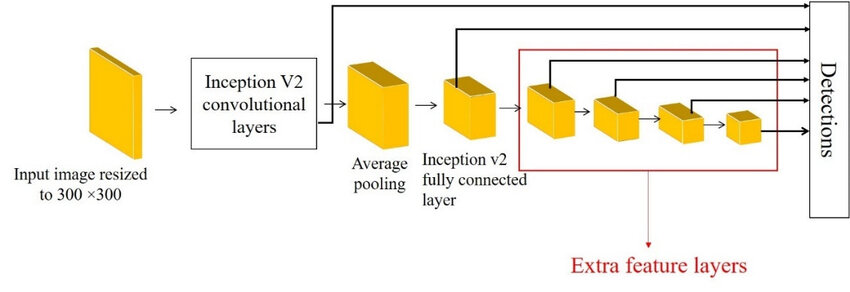
\includegraphics[width=0.85\textwidth]{00Figuras/Single-Shot-Detector-SSD-architecture.jpg}
\caption{Esquema general del detector SSD con predicciones desde múltiples escalas}
\end{figure}

\section{Métodos :}

% ------------------------------------------------------------------
\subsection{Manejo del desbalance de clases}
% ------------------------------------------------------------------

\begin{figure}[H]
    \centering
    \begin{subfigure}[b]{0.48\textwidth}
        \centering
        \includegraphics[width=\textwidth]{00Figuras/distributionLabelsUn.png}
        \caption{Distribución de etiquetas set UN}
        \label{fig:imagen1}
    \end{subfigure}
    \hfill
    \begin{subfigure}[b]{0.48\textwidth}
        \centering
        \includegraphics[width=\textwidth]{00Figuras/distribucionLabelsMelu.png}
        \caption{Distribución de etiquetas set Melbourne}
        \label{fig:imagen2}
    \end{subfigure}
    \caption{Distribución de etiquetas para los sets de datos}
    \label{fig:imagenes}
\end{figure}

Los conjuntos de datos utilizados en este trabajo presentan un marcado desbalance entre
clases: mientras que categorías como \texttt{Mascara\_Descripciones} (UNAL) o
\texttt{database label} (Melbourne) cuentan con miles de instancias etiquetadas, otras
como \texttt{small database label} están notoriamente subrepresentadas. Este desbalance
representa un desafío bien documentado en el entrenamiento de modelos de detección de
objetos~\cite{farrugiaEtAl2022}, pues los optimizadores tienden a sesgar el modelo hacia
las clases mayoritarias, degradando su capacidad de detectar las clases minoritarias.
 
Para mitigar este efecto se adoptaron dos estrategias complementarias. En primer lugar, se
aplicó \textit{data augmentation} dirigido sobre las instancias subrepresentadas, fueron
sometidas a transformaciones geométricas y fotométricas incluyendo rotaciones, cambios de
escala, variaciones de brillo y recortes aleatorios con el fin de incrementar
artificialmente la frecuencia con que estas clases aparecen durante el entrenamiento,
favoreciendo la generalización del modelo sin introducir nuevos datos reales~\cite{Goodfellow2016}.
En segundo lugar, se aprovechó el mecanismo de pesos de clase (\textit{class weights})
implementado de forma nativa en la biblioteca Ultralytics para YOLO: durante el
entrenamiento, el \textit{framework} computa automáticamente un peso inversamente
proporcional a la frecuencia de cada clase en el conjunto de entrenamiento, elevado a una
potencia controlada por el hiperparámetro \texttt{cls\_pw}~\cite{guo2025review}. Este
peso pondera la contribución de cada instancia en la función de pérdida de clasificación,
de modo que los errores cometidos sobre clases raras reciben una penalización mayor y el
modelo dedica proporcionalmente más capacidad de aprendizaje a dichas clases. Adicionalmente,
la función de pérdida focal (\textit{focal loss}) empleada por YOLO reduce la influencia
de las detecciones fáciles predominantemente las de clases mayoritarias amplificando
la señal de gradiente proveniente de los ejemplos difíciles y escasos~\cite{waltonEtAl2023}.
 
% ------------------------------------------------------------------
\subsection{Partición del conjunto de datos: entrenamiento, validación y prueba}
% ------------------------------------------------------------------
 
La partición adecuada de los datos es un paso crítico en el desarrollo de modelos de
aprendizaje profundo, pues de ella depende tanto la capacidad de generalización del modelo
como la validez estadística de las métricas reportadas~\cite{Goodfellow2016}. En este
trabajo se adoptó la proporción \textbf{70\,\%~/ 15\,\%~/ 15\,\%} para
entrenamiento, validación y prueba, respectivamente, siguiendo una práctica ampliamente
establecida en la literatura de detección de objetos~\cite{everingham2010pascal}. Esta
distribución ofrece un equilibrio entre maximizar la cantidad de datos disponibles para el
aprendizaje de los parámetros del modelo y disponer de subconjuntos de evaluación
suficientemente representativos para obtener estimaciones estables de su desempeño.
 
El subconjunto de \textbf{entrenamiento} (70\,\%) concentra la mayor parte de los datos
con el fin de que el modelo pueda aprender la variabilidad morfológica y de disposición
inherente a los artefactos de las láminas de herbario. Para el conjunto de datos UNAL esto
corresponde a 691~imágenes, y para Melbourne a 2\,268~imágenes. Dado que en promedio se
registran cinco etiquetas por lámina, el modelo fue expuesto a aproximadamente
14\,800~instancias de artefactos durante el entrenamiento. Con el propósito de garantizar
que todas las clases minoritarias estuvieran representadas en este subconjunto,
la partición se realizó de forma estratificada, asegurando la inclusión de la totalidad de
las instancias subrepresentadas antes de distribuir el remanente de forma aleatoria.
 
El subconjunto de \textbf{validación} (15\,\%) cumple una función distinta: se emplea
durante el ciclo de entrenamiento para monitorear el desempeño del modelo en datos no
vistos, detectar señales tempranas de sobreajuste y guiar la selección de
hiperparámetros  tasa de aprendizaje, tamaño del lote, número de épocas, entre otros
sin contaminar la evaluación final~\cite{Goodfellow2016}. Por su parte, el subconjunto de
\textbf{prueba} (15\,\%) permanece completamente apartado durante todo el proceso de
desarrollo y es consultado únicamente una vez, al concluir el entrenamiento, con el objeto
de obtener una estimación imparcial del desempeño del modelo ante datos completamente
nuevos~\cite{everingham2010pascal}.
 
% ------------------------------------------------------------------
\subsection{Selección y justificación de las métricas de evaluación}
% ------------------------------------------------------------------
 
La evaluación de modelos de detección de objetos requiere métricas capaces de capturar
simultáneamente la calidad de la clasificación y la precisión de la localización espacial
de los objetos detectados. En este trabajo se seleccionaron tres métricas complementarias:
\textbf{Precisión} (\textit{Precision}), \textbf{puntuación F1} (\textit{F1 score}) e
\textbf{Intersección sobre Unión} (\textit{Intersection over Union}, IoU).
 
La \textit{Precisión} se define como la fracción de detecciones positivas que son
efectivamente correctas:
 
\begin{equation}
  \text{Precisión} = \frac{VP}{VP + FP},
  \label{eq:precision}
\end{equation}
 
\noindent donde $VP$ denota los verdaderos positivos y $FP$ los falsos positivos.
Esta métrica cuantifica la confiabilidad de las detecciones del modelo: un valor alto
indica que la mayoría de los artefactos señalados por el detector corresponden
efectivamente a artefactos reales, minimizando falsas alarmas. En el contexto de la
curaduría de herbarios, una alta precisión es especialmente relevante cuando el objetivo
es verificar la completitud de los artefactos, pues las detecciones espurias podrían
introducir ruido en los reportes automáticos de calidad~\cite{powers2020evaluation}.
 
La \textit{puntuación F1} constituye la media armónica entre la precisión y la
exhaustividad (\textit{recall}):
 
\begin{equation}
  F1 = \frac{2 \cdot \text{Precisión} \cdot \text{Recall}}
            {\text{Precisión} + \text{Recall}},
  \label{eq:f1}
\end{equation}
 
\noindent donde el \textit{recall} mide la fracción de artefactos reales que el modelo
logra detectar ($VP / (VP + FN)$). La puntuación F1 es la métrica más apropiada para
escenarios con clases desbalanceadas~\cite{powers2020evaluation}, como los que caracterizan
a los conjuntos de datos de este trabajo, ya que penaliza por igual los errores de omisión
(artefactos no detectados) y los de comisión (detecciones incorrectas), ofreciendo una
visión integrada y equilibrada del desempeño del modelo por clase.
 
Finalmente, el \textit{IoU} cuantifica el grado de solapamiento espacial entre la caja
delimitadora predicha por el modelo ($B_p$) y la caja delimitadora de referencia ($B_{gt}$):
 
\begin{equation}
  \text{IoU} = \frac{|B_p \cap B_{gt}|}{|B_p \cup B_{gt}|},
  \label{eq:iou}
\end{equation}
 
\noindent y toma valores en el intervalo $[0, 1]$, donde 1 corresponde a un solapamiento
perfecto. Esta métrica es indispensable en tareas de detección de objetos porque evalúa
no solo si el modelo identifica correctamente la categoría del artefacto, sino también
con qué exactitud delimita su posición y extensión en la imagen~\cite{everingham2010pascal}.
Una localización precisa resulta crítica para tareas curatoriales como la ofuscación
de información sensible o la remoción de artefactos previo al análisis morfológico, donde
una caja delimitadora inexacta podría cubrir o exponer inadvertidamente regiones de interés.
En este trabajo se empleó un umbral de $\text{IoU} \geq 0.5$ para determinar si una
detección constituye un verdadero positivo, siguiendo la convención establecida por el
protocolo de evaluación PASCAL VOC~\cite{everingham2010pascal} y adoptada de forma
generalizada en trabajos de detección en imágenes de herbario~\cite{waltonEtAl2023,
hussein2021}.




% Luego se procedió con proceso de selección de la arquitectura apropiada, para esto se realizaron los respectivos entrenamientos por cada modelo y se calculo medidas de confiabilidad y precisión sobre las predicciones del modelo. Las métricas estudiadas con profundidad matemática son:

% \subsection{Recall}
% Mide la capacidad del modelo de identificar todas las instancias positivas presentes:

% \[\text{Recall} = \frac{TP}{TP + FN} = P(\text{predicción positiva} \mid \text{verdad positiva})\]

% donde $TP$ = verdaderos positivos, $FN$ = falsos negativos. Recall alto es crítico en detención de objetos para no perder especímenes.

% \subsection{Precisión}
% Mide qué proporción de predicciones positivas son realmente correctas:

% \[\text{Precisión} = \frac{TP}{TP + FP} = P(\text{verdad positiva} \mid \text{predicción positiva})\]

% donde $FP$ = falsos positivos. Precisión alta minimiza detecciones falsas.

% \subsection{F1-score}
% Media armónica de precisión y recall, proporcionando balance único:

% \[F1 = \frac{2 \cdot TP}{2 \cdot TP + FP + FN} = 2 \cdot \frac{\text{Precisión} \cdot \text{Recall}}{\text{Precisión} + \text{Recall}}\]

% La media armónica penaliza desbalances severos. Es preferred en datasets desbalanceados como el de herbario.

% \subsection{Confianza}
% Representa la probabilidad estimada por el modelo o probabilidad condicional:

% \[\text{Confianza}(c) = P(y=c \mid x) = \text{softmax}(z)_c\]

% Valores > 0.5 típicamente indican detecciones válidas en visión por computadora.

% \subsection{Mean Average Precision (mAP)}
% Métrica estándar para detención de objetos, calculada en dos fases:

% \subsubsection*{Fase 1: Intersección sobre Unión (IoU)}
% Para cada predicción, se computa IoU entre caja predicha y verdad:

% \[\text{IoU} = \frac{\text{Área de intersección}}{\text{Área de unión}} = \frac{|B_{pred} \cap B_{gt}|}{|B_{pred} \cup B_{gt}|}\]

% Predicciones con IoU > umbral (típicamente 0.5) son verdaderos positivos.

% \subsubsection*{Fase 2: Curva Precisión-Recall}
% Para cada clase, se ordena predicciones por confianza decreciente y se computa Average Precision (AP) como el área bajo la curva:

% \[AP = \int_0^1 P(r) \, dr\]

% El mAP es el promedio de AP sobre todas las clases:

% \[mAP = \frac{1}{N} \sum_{i=1}^{N} AP_i\]

%Una vez consideradas estas métricas y con el modelo que mejor se adapte a nuestras necesidades se construyo la arquitectura necesaria para un esquema federado , la cual consiste de un servidor en donde se compilan los pesos de los diferentes modelos desplegados en los clientes, en esta sección se experimento con los principales algoritmos de agregación para el modelo general los cuales son :
\section{Modelo Federado}
 
La inteligencia artificial con arquitectura federada surge como una respuesta a las
crecientes preocupaciones por la privacidad y la seguridad de los datos en el entrenamiento
de modelos de aprendizaje profundo. Su origen se remonta a las investigaciones de Google
en 2016~\citep{mcmahan2017communication}, con el desarrollo de \textit{Federated Learning},
una técnica que permite entrenar modelos directamente sobre los datos de cada participante
sin necesidad de centralizarlos. Esta arquitectura distribuye el proceso de aprendizaje
entre múltiples nodos como teléfonos inteligentes o servidores institucionales que
colaboran para construir un modelo común sin compartir información sensible. A lo largo del
tiempo, la tecnología ha evolucionado incorporando técnicas más avanzadas de agregación de
parámetros, encriptación homomórfica y aprendizaje con privacidad diferencial, lo que ha
reforzado su utilidad en entornos donde la confidencialidad de los datos es
crítica~\citep{bonawitz2016practicalsecureaggregationfederated}.
 
Actualmente, los modelos federados se aplican en sectores como la salud, la banca, las
telecomunicaciones y el internet de las cosas (IoT), donde el acceso a datos distribuidos
es vital y al mismo tiempo restringido. Hospitales, por ejemplo, pueden colaborar para
mejorar modelos de diagnóstico sin intercambiar historiales clínicos de pacientes. El
estado del arte incluye innovaciones como el \textit{federated transfer learning}, que
permite combinar conocimientos de diferentes dominios, y el uso de modelos multimodales
en entornos federados. A pesar de los avances, persisten desafíos técnicos como la
heterogeneidad de los datos, las limitaciones de cómputo en los nodos cliente y la
sincronización eficiente entre rondas. No obstante, la arquitectura federada se consolida
como una de las líneas más prometedoras para un desarrollo ético y escalable de la
inteligencia artificial.
 
% ------------------------------------------------------------------
\subsection{Aprendizaje federado en el contexto de herbarios digitales}
% ------------------------------------------------------------------
 
En el contexto particular de este trabajo, el aprendizaje federado ofrece ventajas
concretas que van más allá de los argumentos generales de privacidad. Los herbarios
digitales operan bajo restricciones institucionales que hacen inviable la centralización
de sus imágenes: los metadatos de localización de especies amenazadas son confidenciales
por razones de conservación; los derechos de imagen sobre los especímenes pertenecen a las
instituciones que los custodian; y los acuerdos de colaboración entre herbarios
frecuentemente prohíben la redistribución de los datos primarios.
 
El aprendizaje federado permite que el \textbf{Herbario Nacional Colombiano (UNAL)} y el
\textbf{University of Melbourne Herbarium} colaboren en el entrenamiento de un detector de
artefactos sin transferir una sola imagen. Adicionalmente, la arquitectura distribuida
habilita dos ventajas operativas de alto valor:
 
\begin{enumerate}
    \item \textbf{Mejora cruzada entre instituciones.} El modelo del nodo UNAL se beneficia
    de los patrones visuales aprendidos sobre los once tipos de artefactos de Melbourne
    escalas, etiquetas impresas, sellos de distintos formatos aunque no los clasifique
    por su nombre local. A la inversa, Melbourne mejora su capacidad de reconocer los
    artefactos característicos del protocolo colombiano. Este intercambio de conocimiento
    visual ocurre sin compartir datos, únicamente a través de los pesos del \textit{backbone}.
 
    \item \textbf{Escalabilidad sin re-etiquetado.} Una tercera institución por ejemplo el
    Kew Gardens o el Smithsonian puede incorporarse al sistema federado entrenando su
    propio nodo con su esquema de etiquetado local, sin necesidad de adaptar ni re-etiquetar
    sus colecciones para hacerlas compatibles con las de los demás participantes.
\end{enumerate}
 
La Figura~\ref{fig:federated_herbarium} ilustra la arquitectura federada adoptada en este
trabajo, en la que cada institución mantiene sus datos y su cabeza de clasificación de
forma local, mientras que el \textit{backbone} del detector se agrega de forma centralizada.
 
\begin{figure}[H]
    \centering
    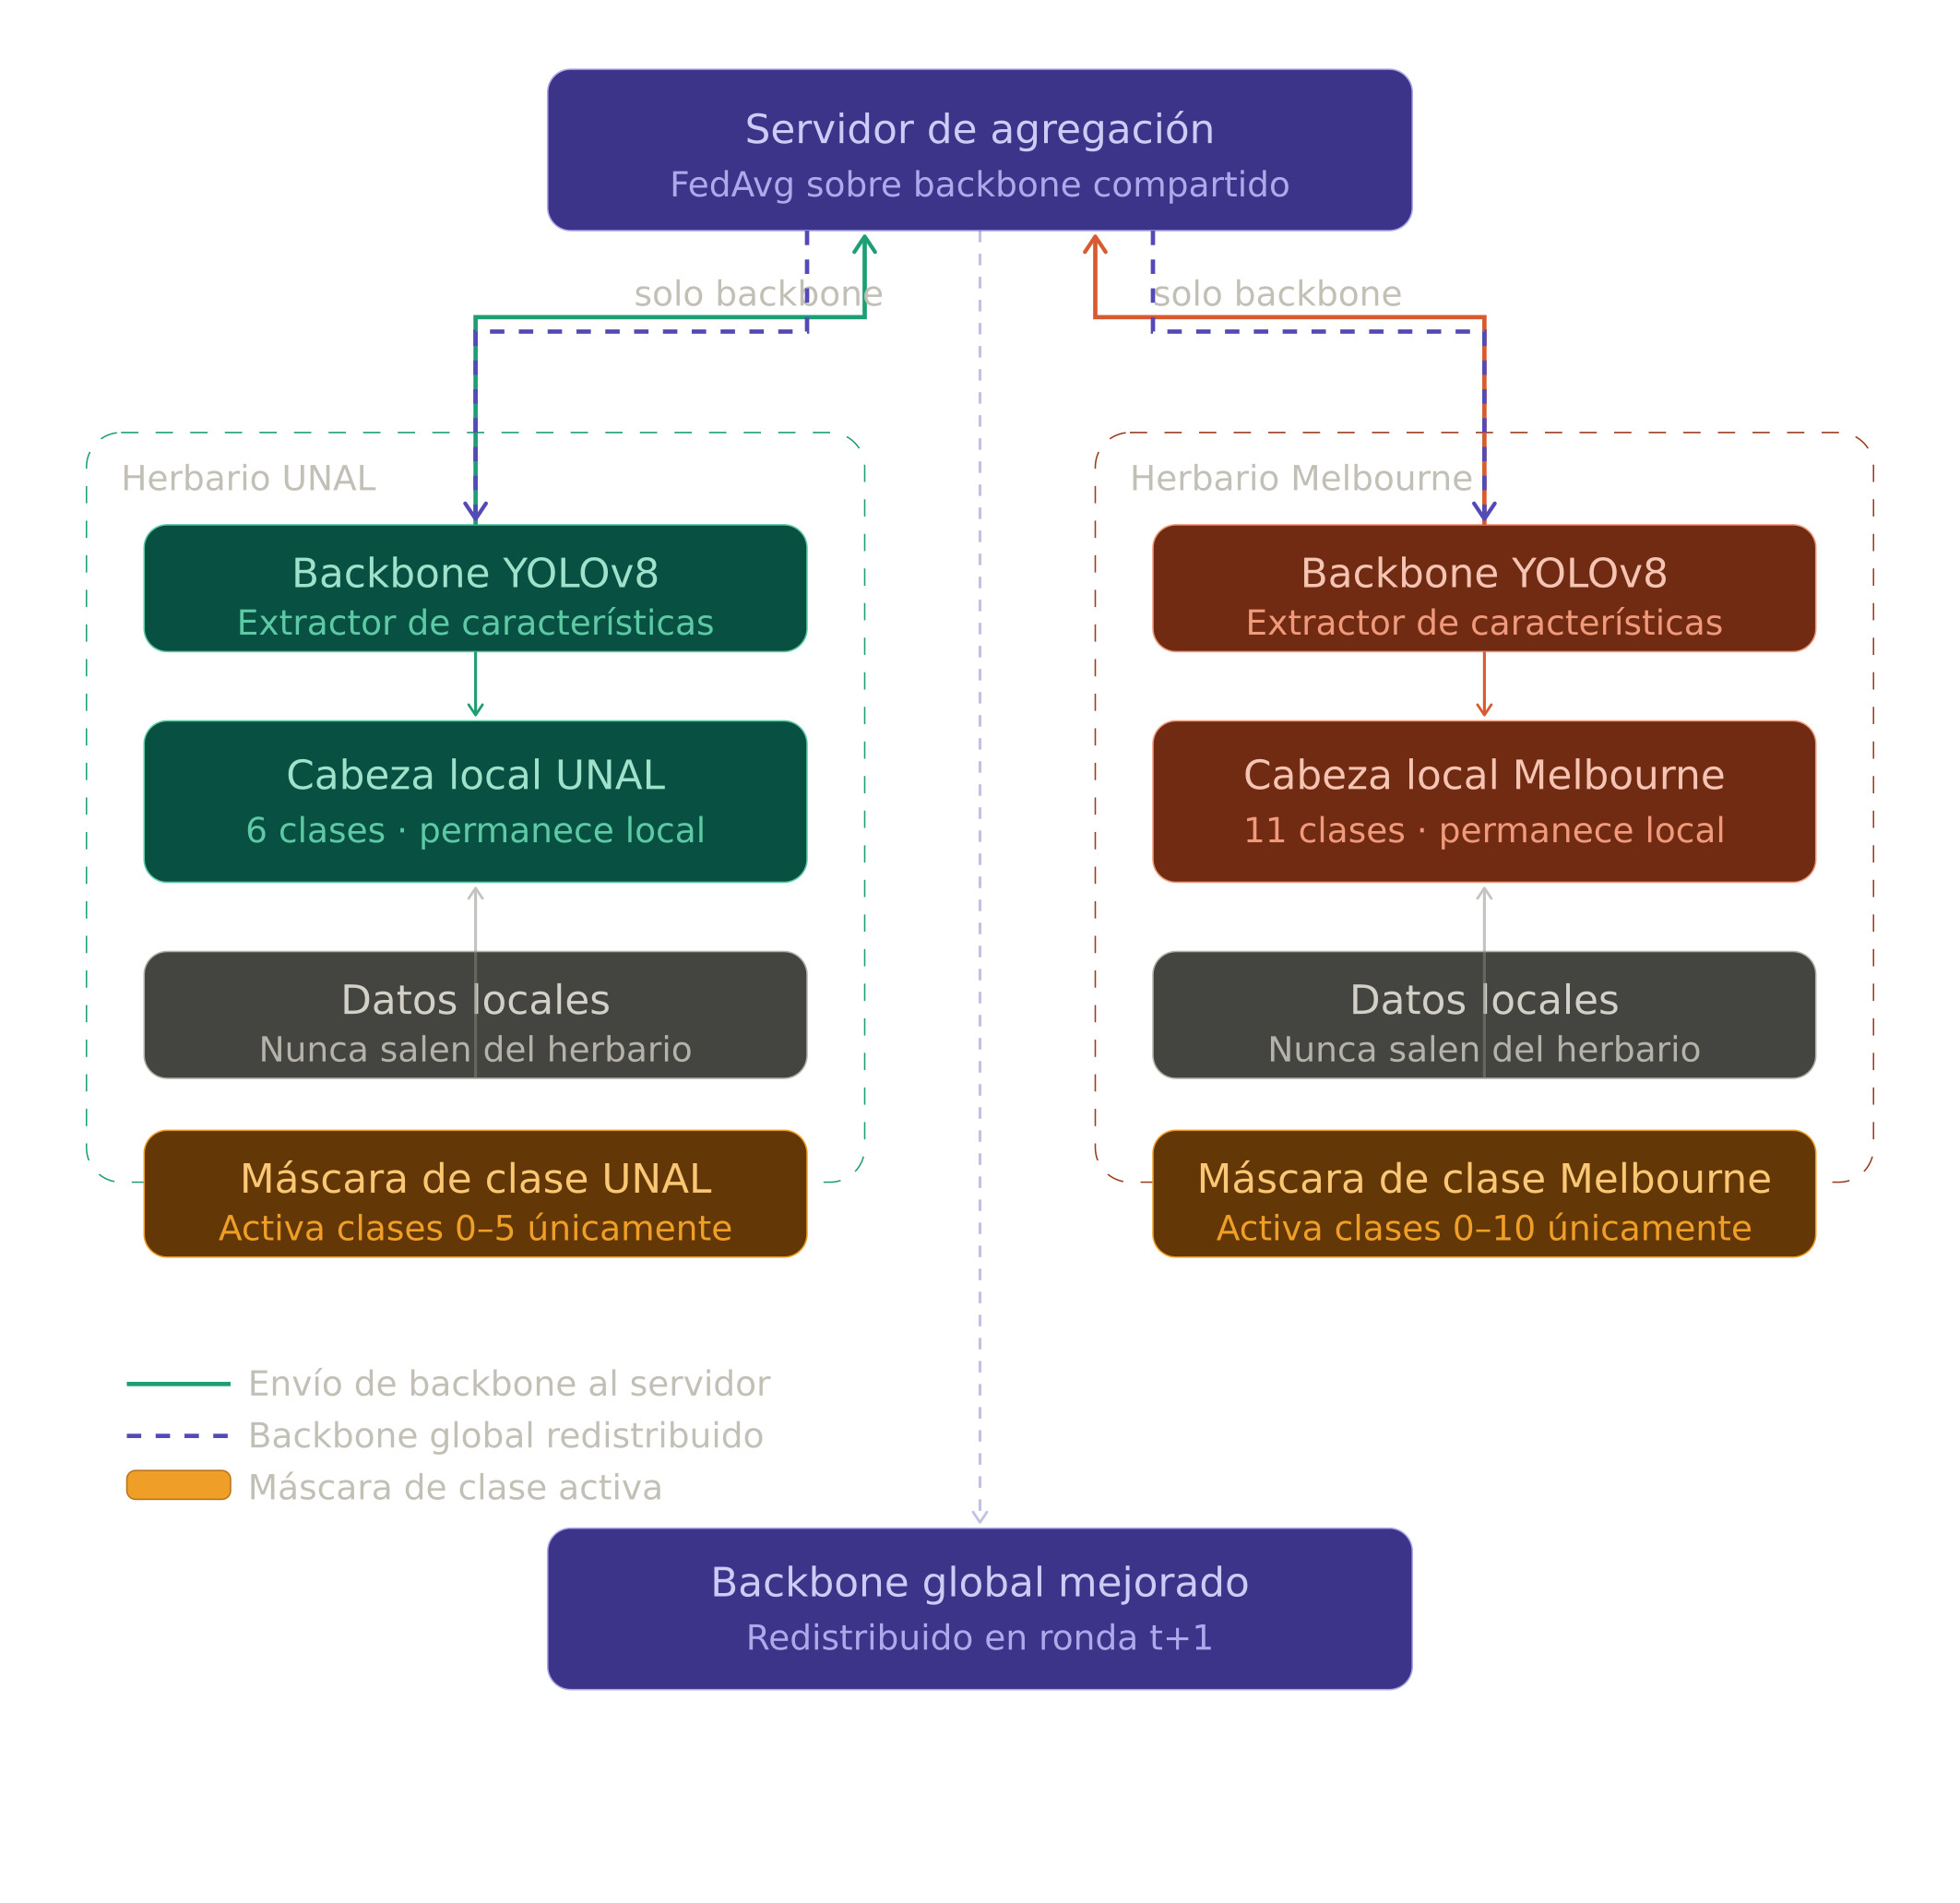
\includegraphics[width=0.92\textwidth]{00Figuras/federated_herbarium_strategy.jpg}
    \caption{Arquitectura federada para la detección de artefactos en registros digitales
             de herbario. Cada nodo institucional (UNAL: 6 clases, Melbourne: 11 clases)
             entrena localmente un modelo YOLOv8 con sus propios datos, que nunca abandonan
             la institución. Solo los pesos del \textit{backbone} el extractor de
             características compartido se envían al servidor de agregación mediante
             FedAvg. Las cabezas de clasificación locales y las máscaras de clase
             (destacadas en naranja) permanecen en cada nodo, evitando la confusión entre
             los vocabularios de etiquetado de ambas instituciones.}
    \label{fig:federated_herbarium}
\end{figure}
 
% ------------------------------------------------------------------
\subsection{Fases del entrenamiento federado}
% ------------------------------------------------------------------
 
El proceso de aprendizaje federado se estructura en fases bien definidas que permiten una
coordinación eficiente entre clientes y servidor:
 
\subsubsection*{Fase 1: Inicialización global}
 
En esta fase inicial, el servidor central genera un modelo global $w_0$ con parámetros
inicializados aleatoriamente. Este modelo es distribuido a todos los clientes
$k \in \{1, 2, \ldots, K\}$, de modo que todos reciben una réplica idéntica:
 
\[
w_0^{(k)} = w_0 \quad \forall\, k
\]
 
\subsubsection*{Fase 2: Entrenamiento local}
 
Cada cliente $k$ realiza un entrenamiento local utilizando únicamente sus datos
$D_k$. Durante $E$ épocas locales, el cliente computa el descenso de gradiente
estocástico:
 
\[
w_t^{(k,e+1)} = w_t^{(k,e)} - \eta \,\nabla F_k\!\left(w_t^{(k,e)}, B\right)
\]
 
donde $w_t^{(k,e)}$ son los parámetros del cliente $k$ en la época local $e$ de la ronda
$t$, $\eta$ es la tasa de aprendizaje local, $B \subset D_k$ es un mini-lote de datos y
$F_k(w) = \frac{1}{|D_k|} \sum_{(x,y) \in D_k} \ell(\mathrm{model}(w, x),\, y)$
es la función de pérdida local. Al completarse las $E$ épocas, el cliente obtiene el modelo
actualizado $w_t^{(k,E)}$.
 
\subsubsection*{Fase 3: Comunicación de parámetros}
 
Cada cliente transmite sus parámetros actualizados $w_t^{(k,E)}$ al servidor central.
En este trabajo se utilizó transmisión sin compresión ($\rho = 1$), aunque es posible
aplicar técnicas de cuantización para reducir el ancho de banda requerido:
 
\[
\tilde{w}_t^{(k)} = \mathrm{Comprime}\!\left(w_t^{(k,E)},\, \rho\right)
\]
 
\subsubsection*{Fase 4: Agregación global}
 
El servidor agrega los parámetros recibidos de todos los clientes mediante uno de los
algoritmos descritos en la Sección~\ref{subsec:agregacion}, produciendo un nuevo modelo
global $w_{t+1}$ que es redistribuido a todos los nodos.
 
\subsubsection*{Fase 5: Criterio de parada}
 
El proceso iterativo se repite hasta cumplirse alguna de las siguientes condiciones:
 
\[
\text{Criterio de parada} =
\begin{cases}
    \text{Continúa} & \text{si } |\mathcal{L}_t - \mathcal{L}_{t-1}| > \varepsilon
                       \;\text{ y }\; t < T_{\max} \\
    \text{Detiene}  & \text{en otro caso}
\end{cases}
\]
 
donde $\mathcal{L}_t$ es la pérdida global promediada en la ronda $t$, $\varepsilon$ es el
umbral de convergencia y $T_{\max}$ es el número máximo de rondas permitidas.
 
% ------------------------------------------------------------------
\subsection{Estrategias para la heterogeneidad de clases entre nodos}
\label{subsec:estrategias_clases}
% ------------------------------------------------------------------
 
El caso concreto de este trabajo presenta un desafío que va más allá del aprendizaje
federado estándar: los dos nodos participantes no comparten el mismo vocabulario de clases.
UNAL emplea seis categorías de artefactos y Melbourne emplea once, con correspondencias
conceptuales parciales pero sin identidad directa (véase la Tabla~\ref{tab:category_mapping_img}).
Esto impide una aplicación directa de FedAvg, que asume que todos los nodos comparten
exactamente la misma arquitectura de salida. A continuación se presentan las tres
estrategias contempladas, en orden creciente de complejidad.
 
\subsubsection{Estrategia 1: Espacio de clases unificado}
 
La aproximación más sencilla consiste en definir un vocabulario global de clases fusionando
los esquemas de ambas instituciones mediante el mapeo conceptual de la
Tabla~\ref{tab:category_mapping_img}. Las once etiquetas de Melbourne se colapsan en los seis
grupos conceptuales de UNAL, de modo que ambos nodos operan con una cabeza de clasificación
idéntica de seis salidas. La agregación FedAvg puede aplicarse sin modificaciones porque
las arquitecturas son plenamente compatibles.
 
La principal limitación de esta estrategia es la pérdida de granularidad: al colapsar
\texttt{small database label}, \texttt{full database label} y \texttt{database label} en
una única clase \textit{Códigos e identificadores}, el modelo pierde la capacidad de
distinguir entre etiquetas de base de datos de distintos tamaños, información que puede
ser relevante para tareas curatoriales específicas de Melbourne.
 
\subsubsection{Estrategia 2: \textit{Backbone} compartido con cabezas locales}
 
Una alternativa más flexible consiste en separar el modelo en dos componentes con
comportamientos distintos durante la federación:
 
\begin{itemize}
    \item \textbf{\textit{Backbone} (capas convolucionales):} aprende representaciones
    visuales generales bordes, texturas, formas independientes del esquema de etiquetado.
    Este componente \emph{sí} se comparte y se agrega mediante FedAvg.
 
    \item \textbf{Cabeza de clasificación:} mapea las representaciones visuales a las clases
    propias de cada institución. Este componente \emph{permanece local} en cada nodo y no
    participa en la agregación.
\end{itemize}
 
La actualización global se restringe entonces al \textit{backbone}:
 
\[
w_{t+1}^{\mathrm{back}} = \sum_{k \in \{\mathrm{UNAL},\,\mathrm{Melb}\}}
    \frac{n_k}{N}\, w_t^{(k,E,\mathrm{back})}
\]
 
La intuición detrás de esta estrategia es que reconocer visualmente un sello institucional
o una escala métrica comparte características de bajo nivel gradientes de color, patrones
de texto, contraste independientemente de cómo se denomine esa clase en cada institución.
El \textit{backbone} federado aprende esas características de forma conjunta; cada nodo las
especializa a través de su propia cabeza. Esta estrategia preserva la granularidad de ambos
esquemas y resulta especialmente atractiva cuando los vocabularios de clase son
substancialmente distintos.
 
\subsubsection{Estrategia 3: Espacio de \textit{embedding} compartido con máscaras de clase}
\label{subsubsec:estrategia3}
 
Esta es la estrategia adoptada en el presente trabajo. En lugar de restringir la
federación al \textit{backbone} o de colapsar los vocabularios, se define un espacio de
salida unificado con $C = C_{\mathrm{UNAL}} + C_{\mathrm{Melbourne}} = 6 + 11 = 17$
clases. El modelo completo incluyendo la cabeza de clasificación tiene arquitectura
idéntica en todos los nodos y participa íntegramente en la agregación FedAvg. La clave que
resuelve el conflicto entre vocabularios es el uso de \textbf{máscaras de clase} durante
el entrenamiento local.
 
Formalmente, para cada cliente $k$, se define una máscara binaria
$m_k \in \{0,1\}^C$ tal que:
 
\[
m_k^{(c)} =
\begin{cases}
    1 & \text{si la clase } c \text{ pertenece al vocabulario del nodo } k \\
    0 & \text{en otro caso}
\end{cases}
\]
 
Durante el cómputo de la pérdida local, el gradiente se anula para las clases
desconocidas en el nodo $k$:
 
\[
\mathcal{L}_k^{\mathrm{masked}}(w) =
    \sum_{c=1}^{C} m_k^{(c)} \cdot
    \ell_c\!\left(\mathrm{model}(w, x),\, y\right)
\]
 
De este modo, el nodo UNAL ($m_{\mathrm{UNAL}}^{(c)} = 1$ para $c \in \{0,\ldots,5\}$)
solo penaliza al modelo por los errores en sus seis clases propias, y el nodo Melbourne
($m_{\mathrm{Melb}}^{(c)} = 1$ para $c \in \{0,\ldots,10\}$) solo penaliza por sus once
clases. Las salidas correspondientes a clases desconocidas en cada nodo no reciben señal
de gradiente y no contaminan el aprendizaje.
 
En inferencia, la institución activa únicamente las salidas de su vocabulario para la
toma de decisiones, ignorando el resto. Esta estrategia presenta tres ventajas respecto a
las anteriores:
 
\begin{enumerate}
    \item \textbf{Preservación total de la granularidad.} Ningún esquema de etiquetado
    es colapsado ni simplificado; ambas instituciones mantienen intacta su taxonomía de
    artefactos.
 
    \item \textbf{Agregación global completa.} A diferencia de la Estrategia~2, la cabeza
    de clasificación también se beneficia de la federación, pues las salidas activas de un
    nodo son indirectamente informadas por las representaciones aprendidas en el otro.
 
    \item \textbf{Extensibilidad natural.} La incorporación de un tercer nodo con un
    vocabulario diferente requiere únicamente definir su máscara $m_k$ y añadir las clases
    nuevas al espacio de salida, sin modificar la arquitectura ni re-entrenar los nodos
    existentes.
\end{enumerate}
 
% ------------------------------------------------------------------
\subsection{Métodos de agregación}
\label{subsec:agregacion}
% ------------------------------------------------------------------
 
La agregación de parámetros constituye el núcleo del aprendizaje federado, permitiendo que
múltiples modelos locales se combinen en un único modelo global. A continuación se presentan
los algoritmos empleados en este trabajo.
 
\subsubsection{Federated Averaging (FedAvg)}
 
FedAvg~\citep{mcmahan2017communication} es el algoritmo fundacional del aprendizaje
federado. Opera mediante un promedio ponderado por la proporción de datos locales:
 
\begin{equation}
    w_{t+1} = \sum_{k=1}^{K} \frac{n_k}{N}\, w_t^{(k,E)}
    \label{eq:fedavg}
\end{equation}
 
donde $n_k = |D_k|$ es el número de muestras en el cliente $k$ y $N = \sum_{k} n_k$.
La ponderación por $n_k / N$ asegura que los nodos con mayor volumen de datos en este
caso Melbourne, con 3\,240 imágenes frente a las 988 de UNAL ejerzan mayor influencia
en la actualización global. Bajo supuestos de convexidad y gradientes acotados, la
convergencia de FedAvg satisface:
 
\[
\mathbb{E}\!\left[\|\nabla F(w_T)\|^2\right] \leq
    \mathcal{O}\!\left(\frac{1}{\sqrt{T}} + \frac{\sigma^2}{K\beta T}\right)
\]
 
donde $\sigma^2$ es la varianza del gradiente y $\beta$ la constante de suavidad.
 
\subsubsection{Federated Stochastic Variance Reduced Gradient (FedSVRG)}
 
FedSVRG mejora FedAvg mediante la introducción de un término corrector de varianza que
mitiga el efecto de la heterogeneidad de datos. En cada cliente $k$, la actualización
local se corrige como:
 
\begin{equation}
    g^{(k)} = \nabla F_k\!\left(w_t^{(k)}\right) -
               \nabla F_k\!\left(\bar{w}_{t-1}\right) + \bar{g}_{t-1}
\end{equation}
 
donde $\bar{g}_{t-1} = \frac{1}{K}\sum_{k} \nabla F_k(\bar{w}_{t-1})$ es el gradiente
promedio global de la ronda anterior. El término corrector
$p^{(k)} = \nabla F_k(\bar{w}_{t-1}) - \bar{g}_{t-1}$ captura la desviación de los
gradientes locales respecto al promedio global, reduciendo la varianza acumulada a:
 
\[
\mathrm{Var}\!\left[g^{(k)}\right] \leq
    \mathcal{O}\!\left(\sigma_{\mathrm{loc}}^2 + \sigma_{\mathrm{global}}^2\right)
\]
 
\subsubsection{FedProx  Federated Proximal}
 
FedProx~\citep{reddi2020adaptive} aborda la heterogeneidad mediante un término
regularizador proximal que mantiene los modelos locales cercanos al modelo global.
La función objetivo en cada cliente se modifica como:
 
\begin{equation}
    \mathcal{L}_k^{\mathrm{FedProx}}(w) =
        \frac{1}{|D_k|} \sum_{(x,y) \in D_k} \ell\!\left(\mathrm{model}(w, x),\, y\right)
        + \frac{\mu}{2}\,\|w - w_t\|_2^2
\end{equation}
 
donde $\mu$ es el coeficiente de regularización proximal. Cuando $\mu \to 0$, FedProx
recupera el comportamiento de FedAvg; a medida que $\mu$ aumenta, las actualizaciones
locales quedan más ancladas al modelo global. FedProx proporciona garantías de convergencia
bajo heterogeneidad fuerte (datos \textit{non-IID}):
 
\[
\mathbb{E}\!\left[\|\nabla F(w_T)\|^2\right] =
    \mathcal{O}\!\left(\frac{1}{T} + \frac{1}{\sqrt{T}}\right)
\]
 
\subsubsection{FedOpt  Optimización federada adaptativa}
 
FedOpt~\citep{reddi2020adaptive} generaliza los métodos de optimización adaptativa (Adam,
AdaGrad) al contexto federado. En lugar de promediar solo los parámetros, FedOpt acumula
momentos de optimización en el servidor:
 
\begin{align}
    m_{t+1} &= \beta\, m_t + (1-\beta)\,\bar{g}_t \\
    w_{t+1} &= w_t - \eta\, m_{t+1}
\end{align}
 
La variante con momentos de segundo orden (Adam federado) incorpora:
 
\begin{align}
    v_{t+1}  &= \alpha\, v_t + (1-\alpha)\,\bar{g}_t^2 \\
    w_{t+1}  &= w_t - \eta\,\frac{m_{t+1}}{\sqrt{v_{t+1}} + \varepsilon}
\end{align}
 
adaptando la tasa de aprendizaje por dimensión, lo que resulta especialmente útil
cuando los gradientes presentan alta variabilidad entre nodos.
 
\subsubsection{FedAvgM  FedAvg con \textit{momentum}}
 
FedAvgM extiende FedAvg incorporando \textit{momentum} en la agregación global, manteniendo
un promedio móvil exponencial de los cambios de parámetros entre rondas:
 
\begin{align}
    m_t      &= \beta\, m_{t-1} + (1-\beta)\left(w_t - w_{t-1}^{\mathrm{agg}}\right) \\
    w_{t+1}  &= w_t + \eta\, m_t
\end{align}
 
O, de forma equivalente:
 
\begin{equation}
    w_{t+1} = w_t + \eta\left[
        \beta\, m_{t-1} + (1-\beta) \sum_{k=1}^{K} \frac{n_k}{N}
        \left(w_t^{(k,E)} - w_t\right)
    \right]
\end{equation}
 
El \textit{momentum} añade inercia a la actualización global, acelerando la convergencia
en direcciones consistentes y atenuando las oscilaciones causadas por la variabilidad entre
rondas. La tasa de convergencia con \textit{momentum} mejora a:
 
\[
\mathbb{E}\!\left[\|\nabla F(w_T)\|\right] =
    \mathcal{O}\!\left(\frac{1}{T^{0.75}}\right)
\]
 
frente a $\mathcal{O}(1/\sqrt{T})$ de FedAvg sin \textit{momentum}.
 
Los resultados experimentales de los algoritmos presentados se discuten en la siguiente
sección.
\chapter{Resultados}

A continuación presentamos los resultados de entrenamiento para los diferentes modelos
y su desempeño en los sets de datos, para luego exhibir algoritmos de agregación en el
modelo federado.

Las siguientes figuras muestran las detecciones realizadas por el modelo fundacional (YOLO) en cada uno de los sets de datos, donde se evidencia una buena capacidad de detección de artefactos. 

\begin{figure}[H]
  \centering
  \vspace{0.5cm}
  \begin{subfigure}[b]{0.48\textwidth}
    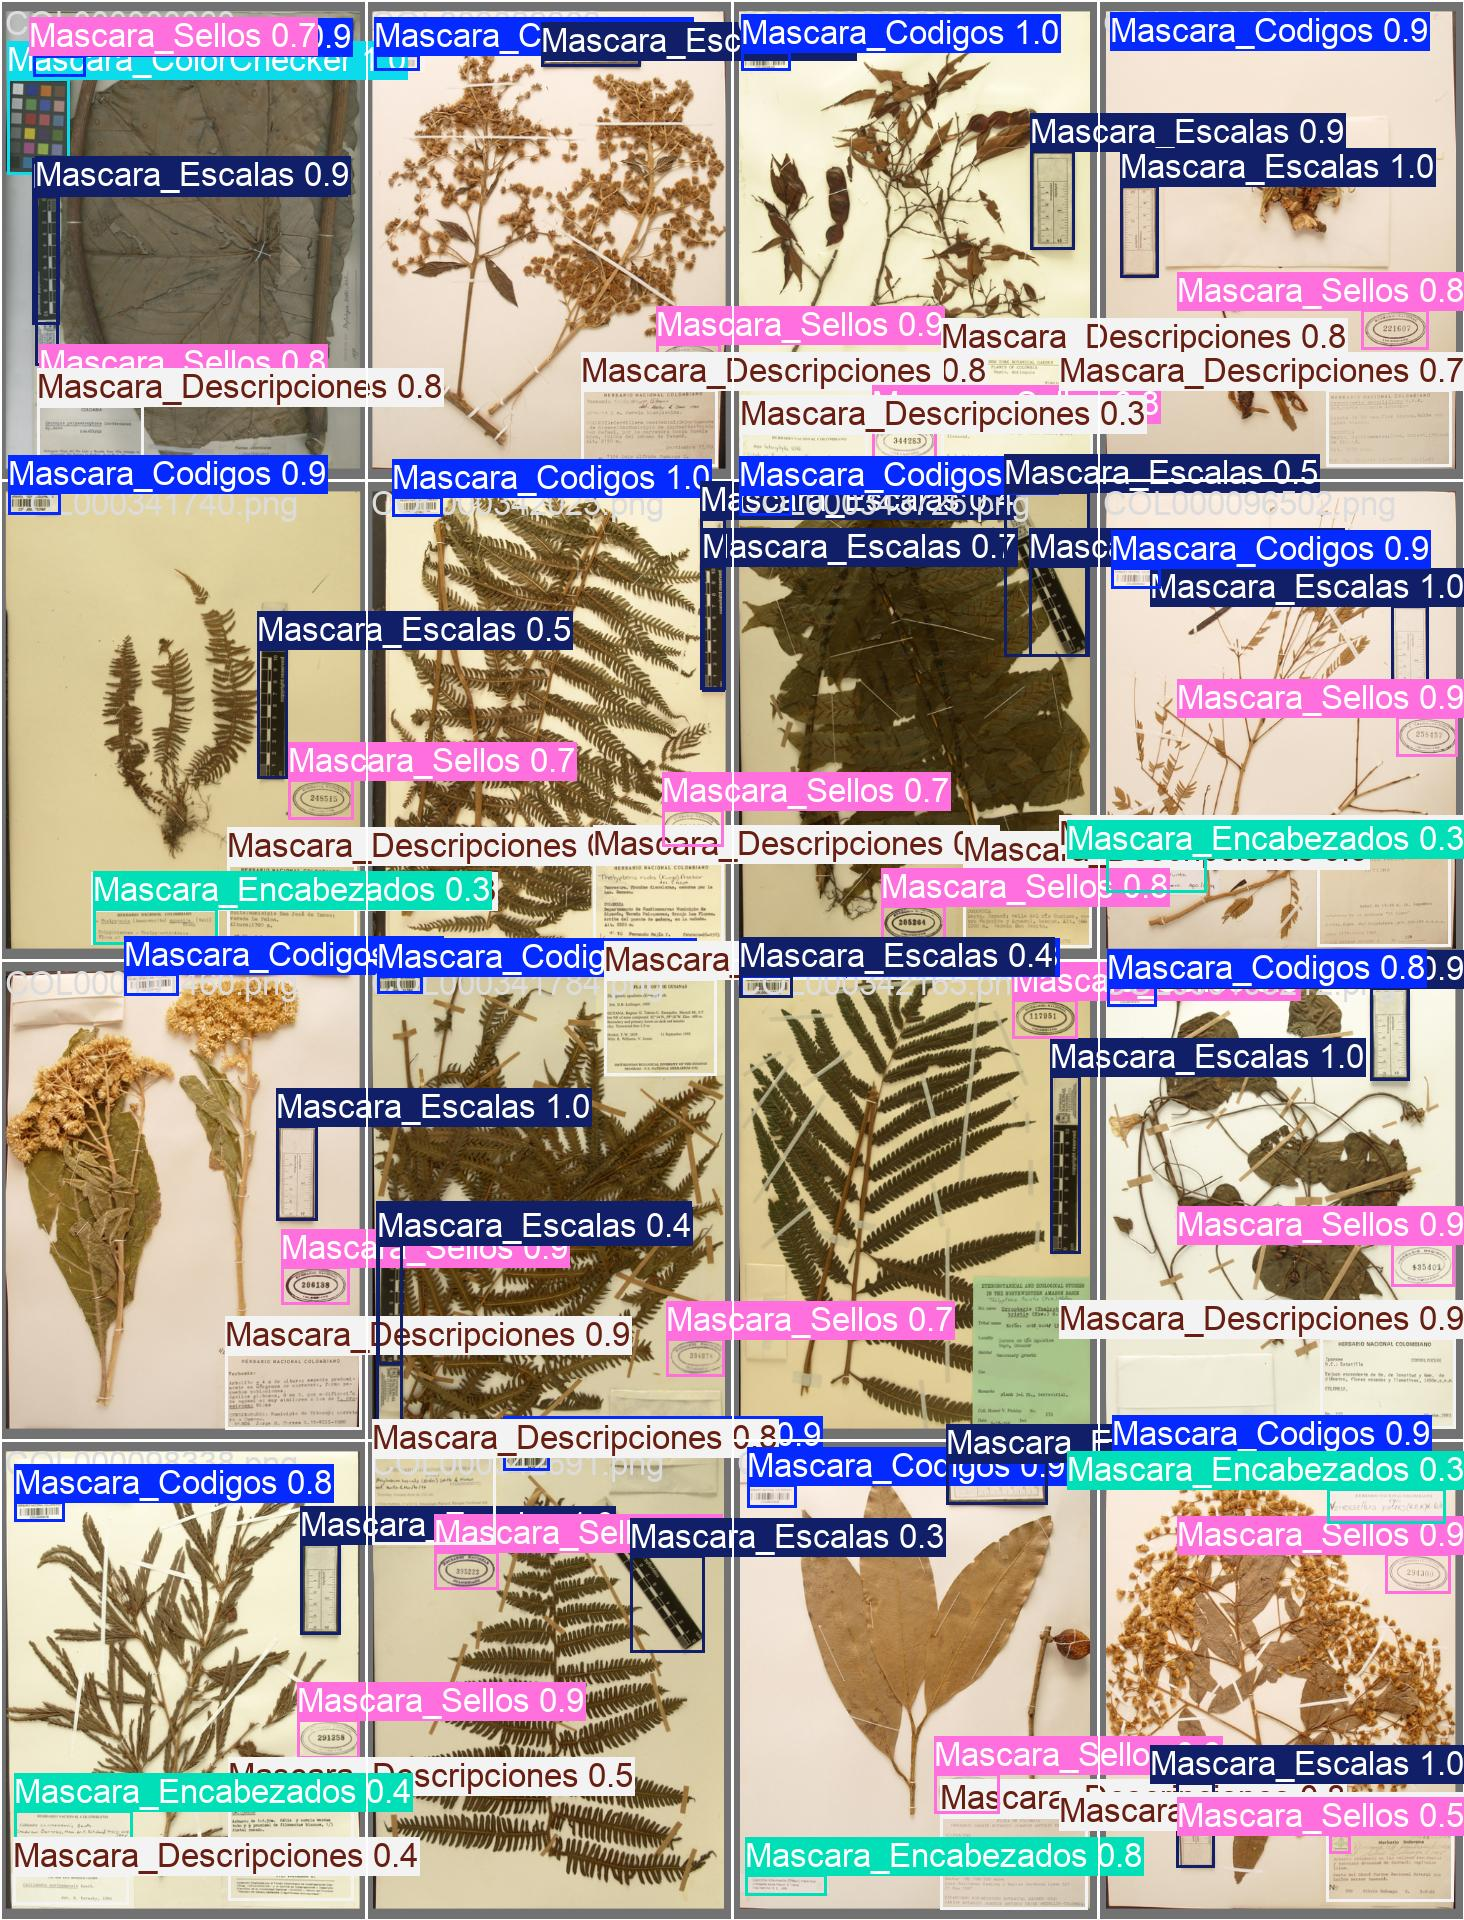
\includegraphics[width=\textwidth]{00Figuras/val_batch0_predClientUn.jpg}
    \caption{Performance de modelo YOLO con datos UN}
    \label{fig:image3}
  \end{subfigure}
  \hfill
  \begin{subfigure}[b]{0.48\textwidth}
    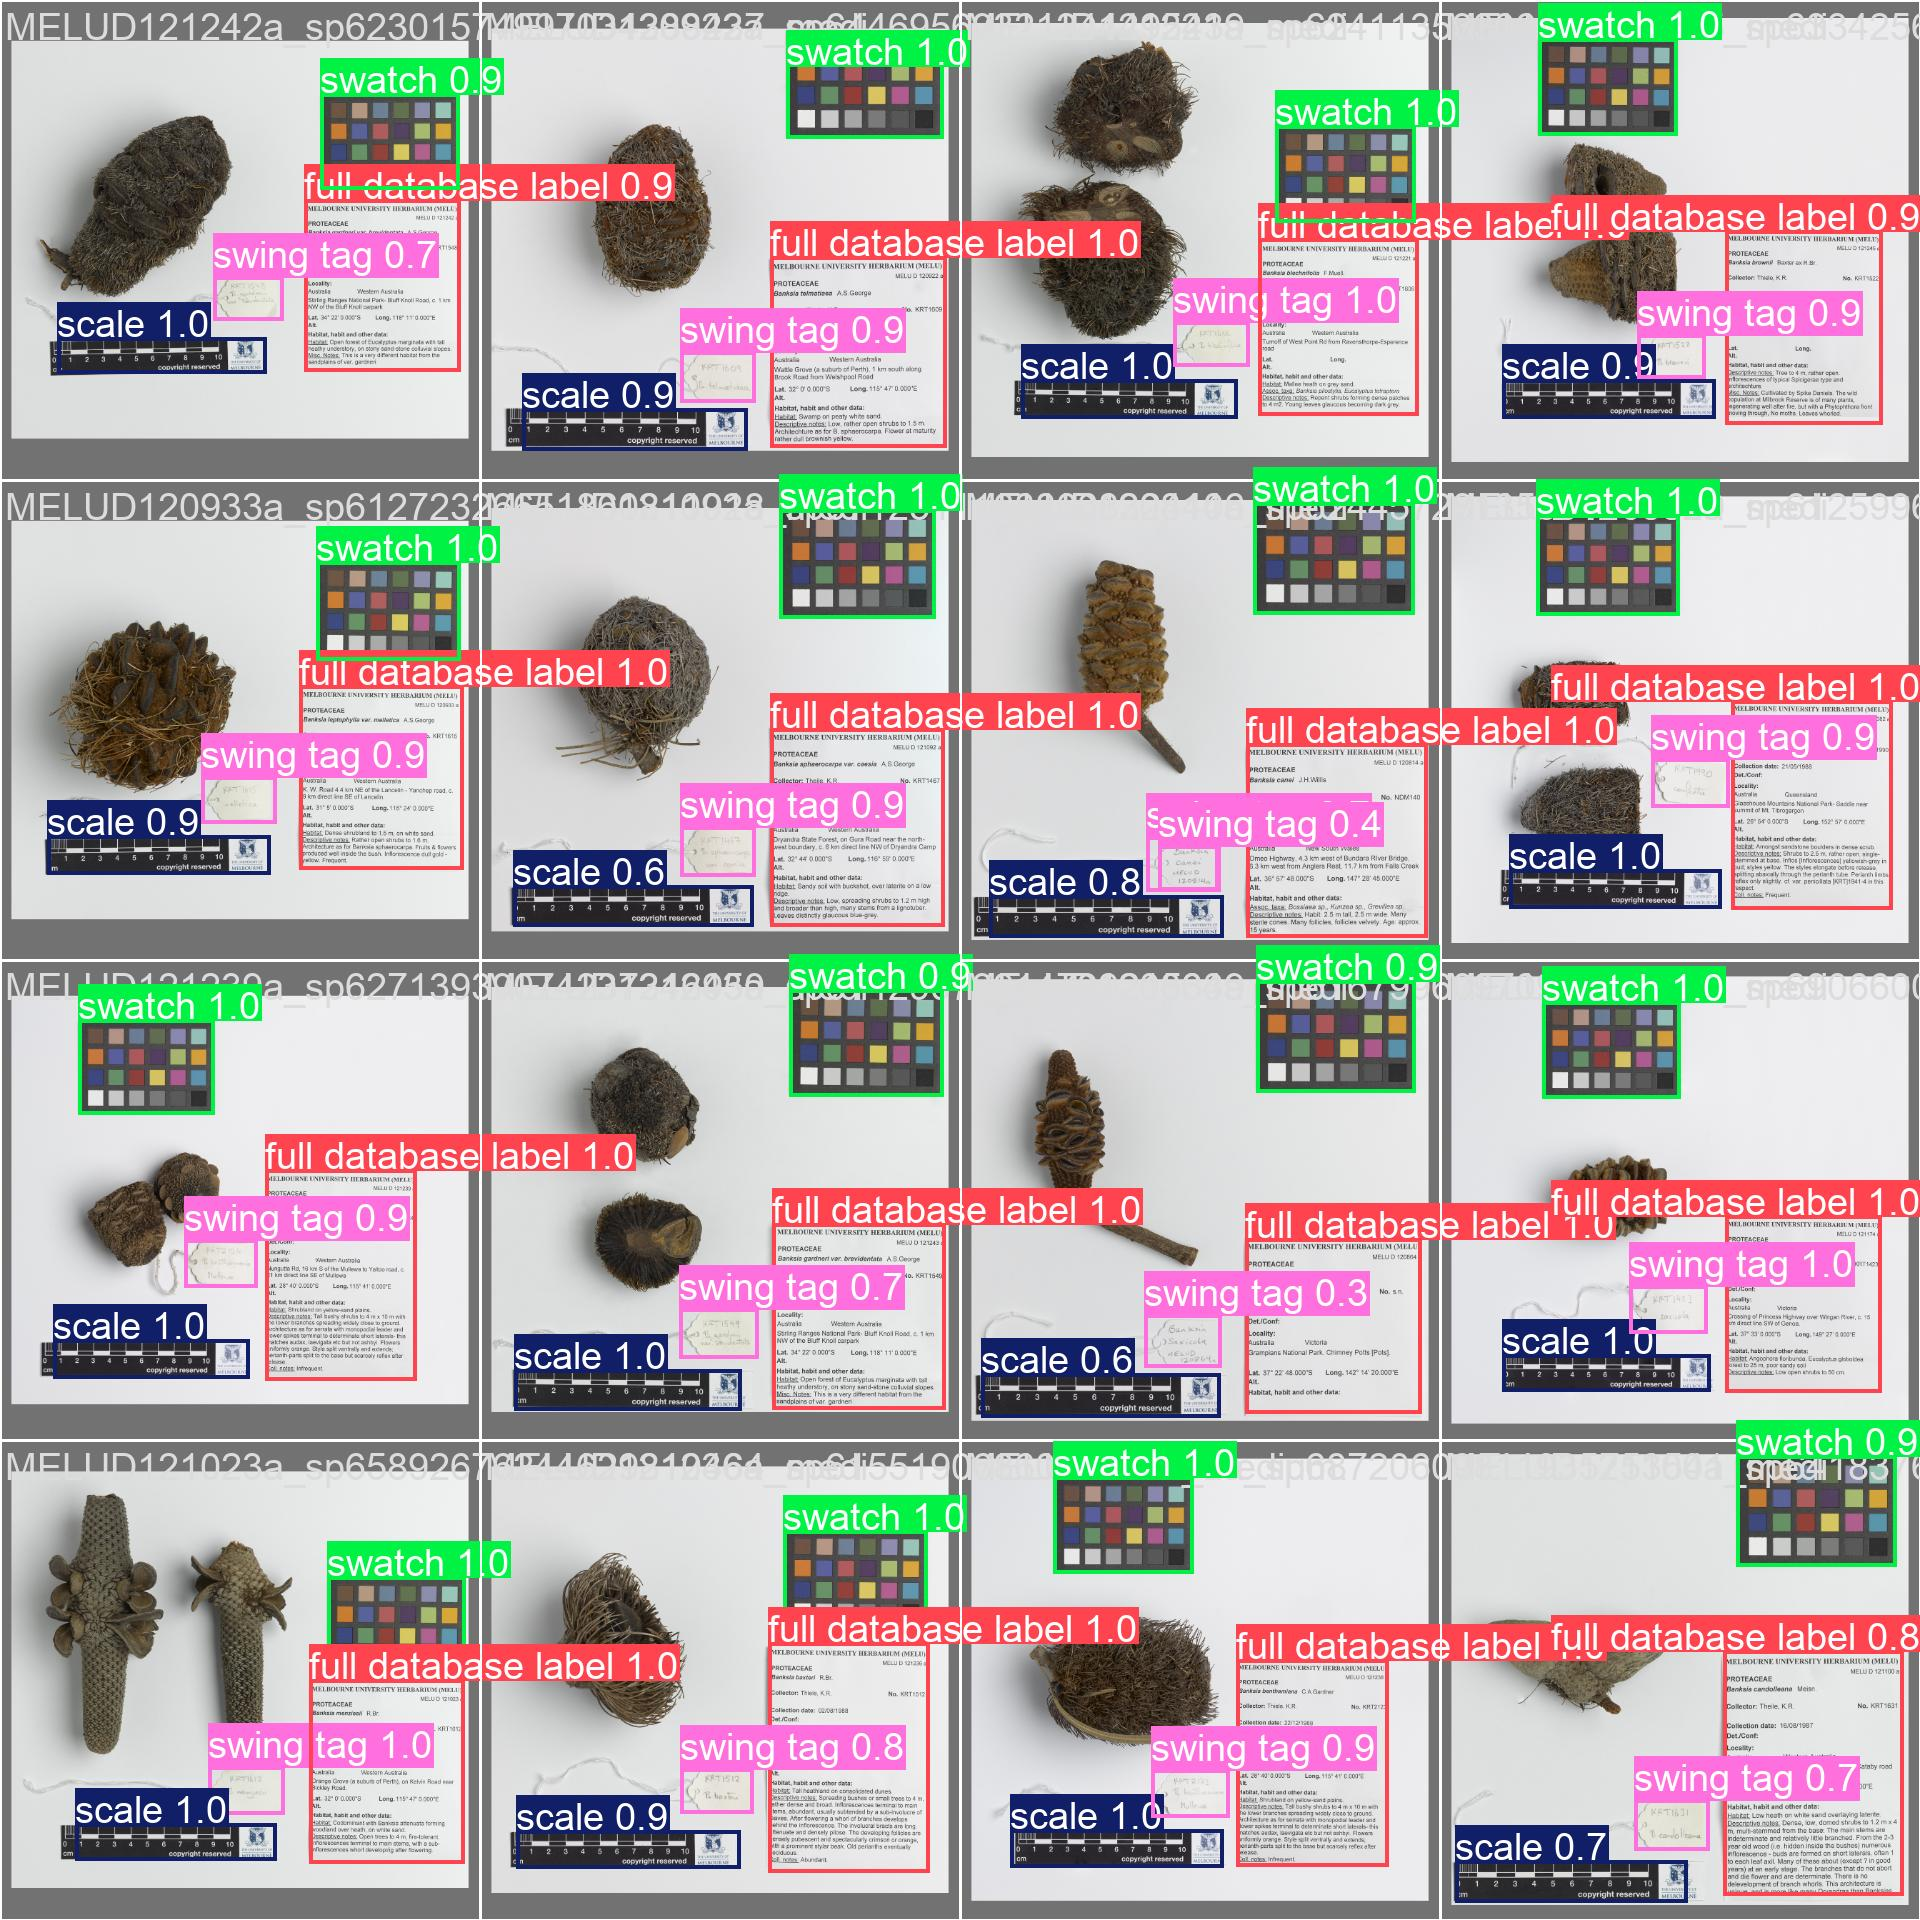
\includegraphics[width=\textwidth]{00Figuras/val_batch1_predMelu.jpg}
    \caption{Performance de modelo YOLO con datos MELU}
    \label{fig:image4}
  \end{subfigure}
  \vspace{0.5cm}
\end{figure}



\section{Primeras detecciones}

La primera etapa del proceso se enfocó en determinar el mejor modelo base para la
arquitectura federada, para ello se hizo uso de las matrices de confusión normalizadas
que en esencia brindan un panorama completo y robusto de cómo está funcionando la tarea
de clasificación para un modelo. A continuación se presentan las matrices asociadas a
los tres modelos considerados.
\begin{figure}[H]
  \centering
  \vspace{0.5cm}
  \begin{subfigure}[b]{0.48\textwidth}
    \includegraphics[width=\textwidth]{00Figuras/lone_confusion_matrix_unal.png}
    \caption{Performance de modelo YOLO con datos UN}
    \label{fig:image3}
  \end{subfigure}
  \hfill
  \begin{subfigure}[b]{0.48\textwidth}
    \includegraphics[width=\textwidth]{00Figuras/lone_confusion_matrix_melu.png}
    \caption{Performance de modelo YOLO con datos MELU}
    \label{fig:image4}
  \end{subfigure}
  \vspace{0.5cm}
\end{figure}

Ahora se presentan las matrices de confusión para el modelo fundacional (YOLO) aplicado las técnicas de aprendizaje federado, donde se evidencia una mejora marginal en la clasificación de artefactos respecto a los modelos individuales.

\begin{figure}[H]
  \centering
  \vspace{0.5cm}
  \begin{subfigure}[b]{0.48\textwidth}
    \includegraphics[width=\textwidth]{00Figuras/confusion_matrix_unal.png}
    \caption{Performance de modelo federado con datos UN}
    \label{fig:image3}
  \end{subfigure}
  \hfill
  \begin{subfigure}[b]{0.48\textwidth}
    \includegraphics[width=\textwidth]{00Figuras/confusion_matrix_melu.png}
    \caption{Performance de modelo federado con datos MELU}
    \label{fig:image4}
  \end{subfigure}
  \vspace{0.5cm}
\end{figure}

De estas se derivó la segunda etapa que fue la de construir una arquitectura federada
capaz de simular el proceso que un herbario debería hacer para poder usar esta
herramienta. A continuación se presentan los resultados del modelo fundacional (YOLO)
aplicado a los distintos sets de datos bajo la modalidad federada de aprendizaje
distribuido; en la siguiente sección se entrará en detalles de la significación de
estos gráficos.

\section{Modelo Federado}

\subsection{Precision Promedio Media (mAP@0.5)}

Presentamos primero un gráfico comparativo del rendimiento de las diferentes estrategias
de agregación, donde se evidencia una ganancia marginal respecto al método de agregación.

\begin{figure}[H]
  \centering
  \begin{tikzpicture}
    \begin{axis}[
      ybar,
      bar width=14pt,
      width=12cm,
      height=7cm,
      ylabel={mAP@0.5},
      xlabel={Algoritmo de Agregación},
      symbolic x coords={FedAvg,FedAvgM,FedProx,FedOpt,FedSVRG},
      xtick=data,
      ymin=0.85, ymax=0.90,
      legend style={at={(0.5,-0.15)},anchor=north,legend columns=2},
      nodes near coords,
      nodes near coords align={vertical},
      enlarge x limits=0.2,
      grid=both
    ]
      \addplot+[fill=blue!50] coordinates {
        (FedAvg,0.886) (FedAvgM,0.886) (FedProx,0.884) (FedOpt,0.885) (FedSVRG,0.885)};
      \addplot+[fill=green!50] coordinates {
        (FedAvg,0.881) (FedAvgM,0.880) (FedProx,0.879) (FedOpt,0.880) (FedSVRG,0.879)};
      \legend{UN, Melbourne}
    \end{axis}
  \end{tikzpicture}
  \caption{Comparación de mAP@0.5 promedio por algoritmo de agregación y conjunto de datos.}
  \label{fig:map_bar}
\end{figure}

Las siguientes métricas se reportan con un \emph{umbral de confianza alto}, donde el
modelo opera en un régimen conservador minimizando falsos positivos.
$\mathrm{mAP}_{50}$ integra precision-recall sobre todas las clases:
\[
  \mathrm{mAP}_{50} = \frac{1}{C}\sum_{c=1}^{C}\int_0^1 p_c(r)\,dr
  \qquad\text{en } \mathrm{IoU} \ge 0.50
\]

\medskip
\begin{table}[H]
  \centering
  \caption{mAP$_{50}$ promedio por estrategia de agregación y conjunto de datos.}
  \small
  \begin{tabular}{lccr}
    \toprule
    \textbf{Algoritmo} & \textbf{UN} & \textbf{Melbourne} & $\Delta$ \textbf{(UN$-$Melb)} \\
    \midrule
    FedAvg  & 0.886 & 0.881 & $+$0.005 \\
    FedAvgM & 0.886 & 0.880 & $+$0.006 \\
    FedProx & 0.884 & 0.879 & $+$0.005 \\
    FedOpt  & 0.885 & 0.880 & $+$0.005 \\
    FedSVRG & 0.885 & 0.879 & $+$0.006 \\
    \midrule
    \textbf{Promedio} & \textbf{0.885} & \textbf{0.880} & $+$0.005 \\
    \bottomrule
  \end{tabular}
\end{table}

\medskip
\begin{table}[H]
  \centering
  \caption{Precision promedio con umbral de confianza alto $\hat{p}_o \ge s_{\text{conf}}^{\text{high}}$.}
  \small
  \begin{tabular}{lccr}
    \toprule
    \textbf{Algoritmo} & \textbf{UN} & \textbf{Melbourne} & $\Delta$ \textbf{(UN$-$Melb)} \\
    \midrule
    FedAvg  & 0.97 & 0.96 & $+$0.01 \\
    FedAvgM & 0.97 & 0.96 & $+$0.01 \\
    FedProx & 0.96 & 0.95 & $+$0.01 \\
    FedOpt  & 0.97 & 0.96 & $+$0.01 \\
    FedSVRG & 0.96 & 0.95 & $+$0.01 \\
    \midrule
    \textbf{Promedio} & \textbf{0.966} & \textbf{0.956} & $+$0.010 \\
    \bottomrule
  \end{tabular}
\end{table}

El Recall se evalúa con un \emph{umbral de confianza bajo}, donde el modelo maximiza
la recuperación de verdaderos positivos al costo de más falsos positivos.
El F1-score balancea ambos regímenes:
\[
  \mathrm{Recall} = \frac{\mathrm{VP}}{\mathrm{VP}+\mathrm{FN}},\qquad
  \mathrm{Precision} = \frac{\mathrm{VP}}{\mathrm{VP}+\mathrm{FP}},\qquad
  F_1 = \frac{2\cdot\mathrm{Precision}\cdot\mathrm{Recall}}{\mathrm{Precision}+\mathrm{Recall}}
\]

\medskip
\begin{table}[H]
  \centering
  \caption{Recall promedio con umbral de confianza bajo $\hat{p}_o \ge s_{\text{conf}}^{\text{low}}$.}
  \small
  \begin{tabular}{lccr}
    \toprule
    \textbf{Algoritmo} & \textbf{UN} & \textbf{Melbourne} & $\Delta$ \textbf{(UN$-$Melb)} \\
    \midrule
    FedAvg  & 0.99 & 0.98 & $+$0.01 \\
    FedAvgM & 0.99 & 0.98 & $+$0.01 \\
    FedProx & 0.98 & 0.98 & $\phantom{+}$0.00 \\
    FedOpt  & 0.99 & 0.98 & $+$0.01 \\
    FedSVRG & 0.98 & 0.97 & $+$0.01 \\
    \midrule
    \textbf{Promedio} & \textbf{0.986} & \textbf{0.978} & $+$0.008 \\
    \bottomrule
  \end{tabular}
\end{table}

\begin{table}[H]
  \centering
  \caption{Máxima puntuación $F_1$ promedio por estrategia de agregación y conjunto de datos.}
  \small
  \begin{tabular}{lccr}
    \toprule
    \textbf{Algoritmo} & \textbf{UN} & \textbf{Melbourne} & $\Delta$ \textbf{(UN$-$Melb)} \\
    \midrule
    FedAvg  & 0.85 & 0.84 & $+$0.01 \\
    FedAvgM & 0.85 & 0.84 & $+$0.01 \\
    FedProx & 0.84 & 0.83 & $+$0.01 \\
    FedOpt  & 0.85 & 0.84 & $+$0.01 \\
    FedSVRG & 0.84 & 0.83 & $+$0.01 \\
    \midrule
    \textbf{Promedio} & \textbf{0.846} & \textbf{0.836} & $+$0.010 \\
    \bottomrule
  \end{tabular}
\end{table}

La brecha consistente $\Delta \in [0.000,\,0.010]$ en todas las métricas y todas
las estrategias confirma que el origen del conjunto de datos (UN vs.\ Melbourne) es una
fuente de varianza mayor que la elección del algoritmo de agregación.
%\chapter{Discusión de resultados}


%El enfoque seguido se basó primero en examinar
%las matrices de confucion y de estas medidas fue posible inferir que el modelo que mejor desepeño tiene en ambos sets de datos en el modelo You Only Look Once (YOLO) \cite{Redmon2016} el cual se usara como piedra angular para la construcción de la arquitectura federada.


%Con el modelo base elegido se construyo una arquitectura federada sencilla en donde se simularon dos clientes y el servidor en donde la agregación de los pesos sera efectuada. Los resultados presentados en la seccion anterior son un conjunto de metricas calculadas en el proceso de validacion y testing del modelo bajo los mencionados algoritmos de agregacion para los modelos federados. El primer resultado directo obtenido a partir de una inspeccion de la forma de las curvas por clase y su comportamiento global, identificando puntos de inflexión o máximos que sugieran umbrales de confianza óptimos. Es que no existe evidencia de una diferencia estadistica significativa entre los algoritmos de agregacion en este set de datos. 

%Posteriormente, se compararon los resultados por clase con la curva promedio (representada en azul en cada gráfico) enfocandonos ya en el comportamiento concreto de las curvas  para tener una idea clara del rendimiento global del modelo y las desviaciones por clase. Finalmente, se interpretaron los valores del mAP@0.5 y otros indicadores directos de desempeño, como la precisión o recall máximo alcanzado, relacionándolos con el tipo de clase y posibles dificultades inherentes a su detección. A partir de esto se 

%\section{Observaciones por gráfico}

%En primer lugar, la curva F1-Confidence muestra cómo varía el balance entre precisión y recall en función del umbral de confianza. Se observa que el modelo logra un máximo F1-score promedio de aproximadamente 0.85 cuando el umbral de confianza es 0.275. Este valor representa el mejor punto de equilibrio global, donde ni la precisión ni el recall predominan, sino que ambos contribuyen equitativamente al rendimiento general. Clases como \textit{Mascara\_Codigos} y \textit{Mascara\_ColorChecker} muestran curvas notablemente altas y planas, lo cual indica un comportamiento robusto a lo largo de distintos niveles de confianza. En contraste, la clase \textit{Mascara\_Encabezados} presenta un F1-score bajo y decreciente, lo cual sugiere que el modelo tiene dificultades tanto para identificar correctamente estas instancias como para evitar falsos positivos.

%Al observar la curva Recall-Confidence, se confirma el comportamiento esperado de que el recall disminuye progresivamente con umbrales más altos de confianza. En el punto extremo de umbral cero, el modelo logra un recall promedio cercano al 0.99, lo que significa que es capaz de detectar casi todas las instancias verdaderas si se permiten predicciones de baja certeza. Nuevamente, las clases de mejor desempeño mantienen altos valores de recall en rangos amplios de confianza, mientras que la clase \textit{Encabezados} muestra un descenso abrupto desde niveles muy bajos de confianza, lo que delata una gran cantidad de falsos negativos incluso con umbrales permisivos.

%La tercera gráfica, Precision-Confidence, revela cómo mejora la precisión a medida que se aumenta el umbral de confianza, sacrificando recall como ya fue visto. El modelo alcanza una precisión promedio de 1.0 cuando la confianza es 1.0, lo cual es natural ya que se están considerando únicamente las predicciones más seguras. Lo más relevante aquí es que el resto de las clases, excepto \textit{Encabezados}, se mantienen en rangos altos de precisión incluso con umbrales bajos, lo que evidencia un modelo confiable en la mayoría de los casos. Sin embargo, la curva de la clase \textit{Mascara\_Encabezados} vuelve a destacar negativamente, ya que parte de una precisión muy baja, por debajo de 0.4, lo que sugiere una alta tasa de falsos positivos.

%Finalmente, la curva de Precisión vs Recall es probablemente la más ilustrativa para visualizar el comportamiento general del modelo. La métrica mAP@0.5 promedio es de 0.886, lo cual representa un rendimiento muy bueno en términos de detección. Las clases \textit{ColorChecker} y \textit{Codigos} tienen un desempeño casi perfecto, con valores superiores a 0.99. Por otro lado, la clase \textit{Encabezados} vuelve a presentar el rendimiento más bajo, con un mAP@0.5 de apenas 0.509, muy por debajo del resto. Esto refuerza la idea de que esta clase específica representa el mayor desafío del modelo y es la principal responsable de la brecha entre el rendimiento ideal y el real.
\chapter{Discusión de resultados}

\section{Comparación con la literatura}

Los resultados obtenidos confirman que la arquitectura \textit{You Only Look Once} (YOLO) \citep{Redmon2016} superó en desempeño a las alternativas evaluadas (RCNN y SSD), alcanzando un mAP@0.5 promedio de 0.886. Este hallazgo concuerda con lo reportado en la literatura, donde YOLO ha mostrado ventajas en detección en tiempo real gracias a su reformulación del problema como regresión directa desde píxeles a coordenadas y categorías, eliminando la necesidad de etapas de propuestas de regiones \citep{Ren2015, Simonyan2014}. Asimismo, la robustez del modelo en clases visualmente regulares como \textit{ColorChecker} y \textit{Códigos} es coherente con estudios que demuestran que la uniformidad estructural de los objetos facilita la generalización \citep{Goodfellow2016, powers2020evaluation}.

En cuanto al aprendizaje federado, la implementación de FedAvg permitió mantener un alto desempeño sin comprometer la privacidad de los datos, tal como lo proponen \citet{McMahan2017} y \citet{bonawitz2016practicalsecureaggregationfederated}. El hecho de que no se observaran diferencias estadísticamente significativas entre algoritmos de agregación (FedAvg, FedProx, FedOpt, FedSVRG) coincide con estudios que indican que, en escenarios de heterogeneidad moderada, FedAvg es suficiente para garantizar estabilidad y convergencia \citep{mansour2022federated, ghosh2020efficient}. No obstante, la literatura también advierte que en contextos con alta variabilidad de los datos, algoritmos más robustos pueden ofrecer ventajas \citep{blanchard2017machine, yin2018byzantine}.

\section{Limitaciones del estudio}

A pesar de los buenos resultados globales, el modelo presenta debilidades claras en la detección de la clase \textit{Encabezados}, cuyo mAP@0.5 apenas alcanzó 0.509. Este bajo desempeño puede atribuirse a factores como: (i) la escasa representación de esta clase en el conjunto de entrenamiento, (ii) la alta variabilidad en tipografías, tamaños y posiciones, y (iii) posibles inconsistencias en las anotaciones. Estas limitaciones se alinean con lo señalado por \citet{sokolova2009systematic} y \citet{huang2007loss}, quienes destacan la dificultad de modelos de clasificación en el tratamiento de clases poco frecuentes o de elevada variabilidad intra-clase.

Adicionalmente, aunque el aprendizaje federado mostró un buen desempeño en este caso, su implementación enfrenta retos prácticos en escenarios reales. Entre ellos destacan la heterogeneidad de hardware en los clientes, la necesidad de sincronización eficiente y los riesgos de convergencia lenta cuando se trabaja con bases de datos mucho más desbalanceadas \citep{reddi2020adaptive}. Por lo tanto, los resultados deben interpretarse como una validación inicial más que como una garantía absoluta de rendimiento en condiciones operativas de mayor complejidad.

\section{Implicaciones para herbarios digitales y perspectivas futuras}

El hallazgo de un umbral de confianza óptimo cercano a 0.275, en el cual se maximiza el F1-score promedio (0.85), resulta particularmente relevante para aplicaciones prácticas de curaduría digital. Este balance entre \textit{precision} y \textit{recall} es crucial en contextos donde los falsos negativos implican pérdida de información taxonómica valiosa. Estudios como los de \cite{chen2020fedbe} resaltan la necesidad de calibrar dinámicamente los umbrales según las prioridades de cada caso de uso, lo cual también sería aplicable a herbarios digitales de diferentes tamaños y recursos.

En términos prácticos, los resultados respaldan el uso de YOLO combinado con aprendizaje federado como una herramienta escalable para la automatización de la curaduría de herbarios. Este enfoque permitiría la integración de colecciones distribuidas sin necesidad de centralizar los datos, favoreciendo la colaboración interinstitucional y garantizando la privacidad de la información, como ya se ha explorado en otros dominios sensibles como la salud y las finanzas \cite{bonawitz2016practicalsecureaggregationfederated,McMahan2017}. 

Finalmente, el estudio abre líneas de investigación futuras: (i) incrementar el tamaño y balance de las clases mediante \textit{data augmentation}, (ii) mejorar la calidad de anotaciones con procesos de curación manual, (iii) explorar arquitecturas modernas con mecanismos de atención espacial \citep{He2016}, y (iv) probar algoritmos de agregación robusta que permitan enfrentar escenarios de datos altamente heterogéneos \citep{mansour2022federated,pillutla2019robust}. De este modo, la propuesta aquí desarrollada puede escalarse y consolidarse como una solución integral para la gestión digital de colecciones botánicas a gran escala.
\chapter{Conclusiones}

A partir del análisis de estas curvas, se concluye que el modelo YOLO presenta un rendimiento excelente para la mayoría de las clases evaluadas, en particular para elementos visualmente distintivos como los códigos QR o los color checkers, cuya estructura visual es clara y constante. El rendimiento general del modelo, con un mAP@0.5 de 0.886, respalda su capacidad para ser utilizado en aplicaciones prácticas sobre imágenes de herbario.

Sin embargo, el modelo presenta claras debilidades en la detección de encabezados. Esta clase muestra valores significativamente inferiores en todas las métricas analizadas, lo cual podría deberse a una baja representación en el conjunto de entrenamiento, anotaciones inconsistentes o alta variabilidad en la forma y posición de los encabezados. Se recomienda reforzar esta clase mediante aumento de datos, curación manual de etiquetas o incorporación de mecanismos de atención espacial más refinados.

Finalmente, el umbral de confianza óptimo para uso práctico se encuentra alrededor de 0.275, permitiendo maximizar el F1-score sin sacrificar demasiada precisión ni recall. Este valor puede utilizarse como referencia para despliegues iniciales, aunque idealmente se debería ajustar dinámicamente según el caso de uso y las prioridades específicas (por ejemplo, minimizar falsos negativos o falsos positivos).
\chapter{Recomendaciones}

Si bien se cuenta con un modelo robusto y capaz de afrontar la tarea de unificar la manera en la que se puede hacer curaduria, como trabajo adicional se propone un esquema que permita estandarizar la forma en la que las muestras son armadas y de esta manera se podria garantizar tasas de acierto (mAP@0.5) por encima del 0.9. al igual que se quiere expandir este modelo a mas herbarios para poder estudiar en comportamiento y consolidar esta herramienta para el uso de toda institucion que requiera este tipo de ayuda 
 
%Inicio del apéndice o anexos
%\begin{appendix}
%\include{08Apendice01}%
%\end{appendix}

%Permite visualizar la bibliografía en la tabla de contenido
%Cambie el nombre a Bibliografía o Literatura Citada en la siguiente línea de ser preciso
\addcontentsline{toc}{chapter}{Referencias Bibliográficas} 

\let\OLDthebibliography=\thebibliography
\def\thebibliography#1{\OLDthebibliography{#1}}
{\scriptsize
\pagestyle{plain}
% Nombre del documento donde se almacenan las referencias
\bibliography{referencias2}
\nocite{*}
% Inserta un página adicional al final en blanco 
%\cleardoublepage
% Para NO insertar una página adicional al final usar \clearpage
\clearpage
}}

\end{document}